\documentclass[a4paper,12pt]{article}
\usepackage{amsmath}
%\usepackage{polish}
\usepackage[polish]{babel}
\usepackage[utf8]{inputenc}
\usepackage[T1]{fontenc}
\usepackage{graphicx}
\usepackage{anysize}
\usepackage{enumerate}
\usepackage{times}
\usepackage{plain}
\usepackage{caption}
\usepackage{graphicx}
\usepackage[space]{grffile}
\usepackage{setspace}
\usepackage{multirow}
\usepackage{datetime}
\usepackage[outputdir=build]{minted}
\usepackage{xcolor}
\usepackage[colorlinks=true]{hyperref}
\usepackage[automake, acronyms, toc, nopostdot, nonumberlist, nomain]{glossaries}
\usepackage{indentfirst}
\hypersetup{
  colorlinks=true,
  linkcolor=blue,
  filecolor=magenta,
  urlcolor=cyan,
}
\urlstyle{same}
%\marginsize{left}{right}{top}{bottom}
\marginsize{2.5cm}{2.5cm}{2.5cm}{2.5cm}
\setlength{\parindent}{4em}
\setlength{\parskip}{1em}
\renewcommand{\baselinestretch}{2.0}

% listings with page breaking
\newenvironment{longlisting}{\captionsetup{type=listing}}{}

\definecolor{bg}{rgb}{0.95,0.95,0.95}
\setminted{
  fontfamily=txtt,
  fontsize=\footnotesize,
  samepage=false,
  style=xcode,
  breaklines,
  bgcolor=bg
}

% custom lexer for toml
\newminted[tomlcode]{../lexers/toml.py:TomlLexer -x}{}
\newmintinline[tomlcodeinline]{../lexers/toml.py:TomlLexer -x}{}
\newmintedfile[tomlfile]{../lexers/toml.py:TomlLexer -x}{}

% custom lexer for ladr
\newminted[ladrcode]{../lexers/ladr.py:LadrLexer -x}{}
\newmintinline[ladrcodeinline]{../lexers/ladr.py:LadrLexer -x}{}
\newmintedfile[ladrfile]{../lexers/ladr.py:LadrLexer -x}{}

% custom lexer for spass
\newminted[spasscode]{../lexers/spass.py:SpassLexer -x}{}
\newmintinline[spasscodeinline]{../lexers/Spass.py:SpassLexer -x}{}
\newmintedfile[spassfile]{../lexers/spass.py:SpassLexer -x}{}

% custom lexer for tptpt
\newminted[tptpcode]{../lexers/tptp.py:TptpLexer -x}{}
\newmintinline[tptpcodeinline]{../lexers/tptp.py:TptpLexer -x}{}
\newmintedfile[tptpfile]{../lexers/tptp.py:TptpLexer -x}{}

\loadglsentries{../glossaries}
\makeglossaries
\glsaddall

\begin{document}
\onehalfspacing
\begin{figure}[!htb]
  \centerline{
\includegraphics[scale=0.8]{../images/agh_logo.jpg}}
\end{figure}

\begin{center}
  \Huge{Studio projektowe 1\\}
  \Large{Benchmark solverów prover9 oraz SPASS\\ \large \textit \today \\}
  \vspace{3cm}
  \Large{	Autorzy:\\
    Mateusz Grzeliński\\
    Przemysław Michałek\\
  }
  \large{Wydział Elektrotechniki, Automatyki, Informatyki i Elektroniki}

  \newpage
\end{center}

\tableofcontents
\newpage

\section{Wprowadzenie}

Celem projektu jest zbadanie wydajności automatyczych metod dowodzenia twierdzeń Prover9 oraz SPASS w kontekście formuł żywotnościowych i bezpieczeństwa, przedstawionych jako problem \gls{SAT}, a dokładniej \gls{FOF}. Na początku zostaje wygenerowna formuła \gls{SAT}, która zostaje rozwiązana przez badane provery. Badany jest czas wykonania, rezultat (czy \gls{SAT} jest spełnialny), użycie pamięci RAM.  Generowana formuła \gls{SAT} jest modyfikowana ze względu na między innymi długość formuły, ilość zmiennych.

Provery traktowane są jako czarne skrzynki (blackbox), ich parametry są modyfikowane z poziomu linii komend.

\subsection{Żywotność i bezpieczeństwo formuł}

\textbf{Żywotność} systemu to cecha, która zapewnia, że coś dobrego na pewno w końcu się wydarzy. Formuła żywotnościowa gwarantuje, że istnieje co najmniej jedno wydarzenie, dla którego formuła będzie spełniona.

\textbf{Bezpieczeństwo} systemu to cecha, która zapewnia, że nic złego nigdy się nie stanie. Formuła bezpieczeństwa gwarantuje, że dla każdego wydarzenia, formuła bezpieczeństwa nigdy nie zostanie pogwałcona.

Żywotność oraz bezpieczeństwo mogą zostać wyrażone na przykład w postaci formuły logicznej pierwszego rzędu, czyli problemu SAT.
W formacie TPTP formuły żywotnościowe i bezpieczeństwa można przedstawić jako:
\begin{itemize}
  \item kwantyfikatory (\gls{FOF}) - w tptp kwantyfikator uniwersalny to \mintinline{text}{!}, a kwantyfikator egzystencjalny \mintinline{text}{?}
  \item kaluzule \gls{CNF} - powstaje po przekonwertowaniu formuły z kwantyfikatorem w klazulę
\end{itemize}

\begin{tptpcode}
fof(simple_exists, axiom,
 ? [W,Z] :  p(W, Z) | p(a, b)
  ).

% converted with TPTP2X, otter algorithm
cnf(simple_exists_1,axiom,
    ( p(sk1,sk2) | p(a,b) )).
\end{tptpcode}

\begin{tptpcode}
fof(simple_for_all, axiom,
 ! [W,Z] :  p(W, Z) | p(a, b)
  ).

% converted with TPTP2X, otter algorithm
cnf(simple_for_all_1,axiom,
    ( p(A,B) | p(a,b) )).
\end{tptpcode}

\begin{tptpcode}
% dla każdego X, Y operacja lesseq, to to samo co less lub równość
fof(this_is_obvious, axiom,
  ! [X,Y] : ( $lesseq(X,Y) <=> ( $less(X,Y) | X = Y ) )
  ).

% converted with TPTP2X, otter algorithm
cnf(this_is_obvious_1,axiom,
    ( ~ $lesseq(A,B) | $less(A,B) | A = B )).

cnf(this_is_obvious_2,axiom,
    ( ~ $less(A,B) | $lesseq(A,B) )).

cnf(this_is_obvious_3,axiom,
    ( A != B | $lesseq(A,B) )).
\end{tptpcode}

\begin{tptpcode}
fof(combined, axiom,
 ? [W,Z] : ( ! [X, Y] : p(W, Z, X)  | d(Y) )
  ).

% converted with TPTP2X, otter algorithm
cnf(combined_1,axiom,
    ( p(sk1,sk2,A) | d(B) )).
\end{tptpcode}

\subsubsection{Przykład: zdawanie egzaminu}

\noindent
Problem: zalicz egzamin, aby zdać kurs

\noindent
Warunek bezpieczeństwa: jeżeli podejmujesz się egzaminu, zalicz go

\noindent
Warunek żywotnościowy: kiedyś musisz podejść do egzaminu

\subsubsection{Przykład: światła na skrzyżowaniu}

\noindent
Problem: samochody chcą przejechać przez skrzyżowanie

\noindent
Warunek bezpieczeństwa: tylko jedno światło powinno być zielone

\noindent
Warunek żywotnościowy: każde światło powinno kiedyć zmienić się na zielone


\section{Benchmark}

Problem benchmarku w strategii blackbox sprowadza sie do wykonania podprogramu z odpowiednimi opcjami z poziomu linii komend.
Wejście oraz testy benchmarka ustawiane są poprzez plik konfiguracyjny, sekcja \ref{benchmarkUsage}.  Wejściem testu jest zbiór formuł \gls{SAT} zapisanych na dysku w formacie TPTP w postaci pliku tesktowego. Test polega na podaniu pliku TPTP do provera. W razie potrzeby nastąpi automatyczna konwersja do odpowiedniej składni za pomocą dostępnych translatorów.
Dla każdego provera dostępne są statystyki:

\begin{itemize}
  \item czas wykonania
  \item użycie pamięci RAM
  \item spełnialność formuły
\end{itemize}

\noindent
Więcej statystyk może zostać zebrany przez parser, który bada wyjście provera (sekcja \ref{parser}).
\newline
Zbadane zostaną statystyki proverów ze względu na następujące właściwości formuły SAT:

% more here:http://www.tptp.org/TPTP/TR/TPTPTR.shtml#ProblemGenerators
\begin{itemize}
  \item SAT type (CNF, FOF)
  \item number of clauses (CNF) - w składni TPTP jest to liczba użytych słów \mintinline{text}{cnf}
  \item number of atoms - ilość literałów połączonych operatorem \textit{lub}
  \item maximal clause size
  \item number of predicates - predykat ustanawia n-argumentową relację między argumentami
  \item number of functors
  \item number of variables - ilość atomów, które zaczynają się dużą literą. Jeśli zmienna \textit{X} wystąpi w dwóch różnych klauzulach, traktowana jest jako 2 różne zmienne
  \item maximal term depth
\end{itemize}

Example in tptp syntax:

\begin{tptpcode}
% total in this example: 2 clauses, 6 atoms, 4 predicates, 1 functor, 2 variables

% clause: 4 atoms, 4 predicates, 0 functors, 1 variable
cnf(predicates_examples, axiom,
  ( 'p 1' % arity 0
  | p2
  | 'p 3'(X) % arity 1, variable X
  | p4(y) % arity 1, fact y
  )).

% clause: 2 atoms, 1 predicate, 1 functor, 1 variable
cnf(clause2, negated_conjecture,
    ( p4(X)
    | p4(f(X)) % f(X) is a functor
    )).

\end{tptpcode}

\begin{figure}[H]
  \centering
  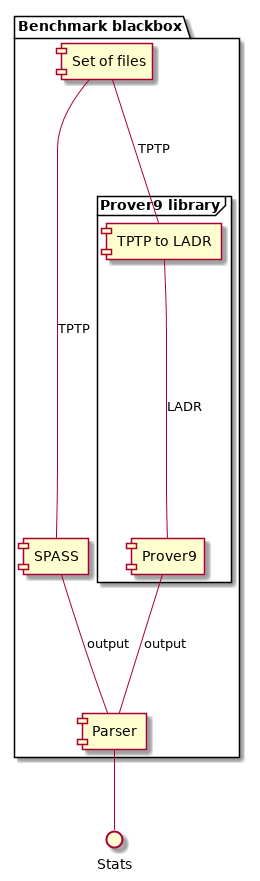
\includegraphics[scale=0.5]{benchmark/components.png}
  \caption{Diagram komponentów systemu benchmarka}
\end{figure}

\subsection{Prover9}

Prover9 jest to zautomatyzowane narzędzie udowadniające dla logiki pierwszego rzędu stworzone przez Williama McCune’a.

Prover9 dostępny jest jako plik wykonywalny, przyjmuje pliki w formacie \gls{LADR}. Dla uniwersalności zostanie zastosowany konwerter TPTP do LADR dostępny wraz z Proverem9 jako osobny plik wykonywalny. Ilość opcji dostępnych z lini komend jest minimanlna, jedyną ważną opcją z punktu widzenia benchmarka jest \mintinline{text}{-x - set(auto2).  (enhanced auto mode)}

\noindent
Oficjalna strona internetowa \url{https://www.cs.unm.edu/~mccune/mace4/}

\begin{longlisting}
  \caption{Przykład pliku wejściowego w składni LADR}
  \ladrfile{listings/prover9_example.in}
\end{longlisting}

\begin{longlisting}
  \caption{Przykład wyjścia Provera9}
  \inputminted{text}{listings/prover9_example.out}
\end{longlisting}

\subsubsection{TPTP to LADR}

W bibliotece \gls{LADR}, która jest załączona wraz ze źródłami Provera9, dostępny jest translator składni TPTP do LADR. Jest to plik wykonywalny. Na standardowe wejście przyjmuje TPTP, na standardowy wyjście podaje LADR.

Alternatywą do konwertera dostarczanego razem z prover9 jest program \mintinline{text}{tptp2X} dostarczanego przez TPTP.

\subsection{SPASS}

SPASS Theorem Prover jest narzędziem do automatycznego dowodzenia twierdzeń, należących do rachunku predykatów pierwszego rzędu.

SPASS nie korzysta z zewnętrznych bibliotek, dostępny jest jako plik wykonywalny. Akceptuje pliki w składni TPTP lub swojej własnej. SPASS udostępnia wiele opcji z poziomu lini komend. Z punktu widzenia benchmarka istotnymi są:

\begin{itemize}
  \item TODO
\end{itemize}

\noindent
Wszystkie opcje linii komend \url{https://webspass.spass-prover.org/help/options.html}
\noindent \newline
Oficjana strona internetowa \url{https://webspass.spass-prover.org/}

\begin{longlisting}
  \caption{Przykład pliku wejściowego w składni SPASS}
  \spassfile{listings/spass_example.in}
\end{longlisting}

\begin{longlisting}
  \caption{Przykład wyjścia SPASS}
  \inputminted{text}{listings/spass_example.out}
\end{longlisting}

\subsection{TPTP}

TPTP - \textit{ang. (Thousands of Problems for Theorem Provers)} - to biblioteka problemów wykorzystywanych do testowania systemów \gls{ATP}. Jednocześnie jest to nazwa formatu, w którym zapisywane są te testy. TPTP udostępnia te problemy na oficjalnej stronie intenetowej. Razem z TPTP istnieje TSTP (\textit{ang. Thousands of Solutions from Theorem Provers}) - biblioteka rozwiązań problemów.
Te problemy są sklasyfikowane przez domeny (3 literowe skróty), przykładowo LCL - Logic Calculi, COL - Combinatory Logic

W formacie TPTP można zapisywać \gls{TPI}, \gls{THF}, \gls{TFF}, \gls{FOF}, \gls{CNF}. Celem benchmarka jest badanie proverów logiku pierwszego rzędu, więc interesują nas \gls{CNF}, \gls{TFF}, \gls{FOF} (TFF/FOF with external clausifiers).

% from technical manual http://www.tptp.org/TPTP/TR/TPTPTR.shtml
\subsubsection{Wybrane elementy składni TPTP}

\begin{itemize}
  \item The syntax for atoms is that of Prolog: variables start with upper case letters, atoms and terms are written in prefix notation, uninterpreted predicates and functors either start with lower case and contain alphanumerics and underscore, or are in 'single quotes'.

  \item Each logical formula is wrapped in an annotated formula structure of the form  \newline \mintinline{text}{language(name,role,formula,source,[useful_info])}

    \begin{itemize}
      \item role gives the user semantics of the formula, one of
        \mintinline{text}{axiom},
        \mintinline{text}{hypothesis},
        \mintinline{text}{definition},
        \mintinline{text}{assumption},
        \mintinline{text}{lemma},
        \mintinline{text}{theorem},
        \mintinline{text}{corollary},
        \mintinline{text}{conjecture},
        \mintinline{text}{negated_conjecture},
        \mintinline{text}{plain},
        \mintinline{text}{type},
        and \mintinline{text}{unknown}.  Axiom-like formulae are those with the roles
        \mintinline{text}{axiom},
        \mintinline{text}{hypothesis},
        \mintinline{text}{definition},
        \mintinline{text}{assumption},
        \mintinline{text}{lemma},
        \mintinline{text}{theorem},
        and \mintinline{text}{corollary}. They are accepted, without proof, as a basis for proving conjectures in THF, TFF, and FOF problems. In CNF problems the axiom-like formulae are accepted as part of the set whose satisfiability has to be established. \mintinline{text}{conjecture} occur in only THF, TFF, and FOF problems, and are to all be proven from the axiom(-like) formulae. A problem is solved only when all conjectures are proven. TPTP problems never contain more than one conjecture. \mintinline{text}{negated_conjectures} are formed from negation of a \mintinline{text}{conjecture}, typically in FOF to CNF conversion.
      \item The \mintinline{text}{useful_info} field of an annotated formula is optional, and if it is not used then the \mintinline{text}{source} field becomes optional. The \mintinline{text}{source} field is used to record where the annotated formula came from, and is most commonly a file record or an inference record.
    \end{itemize}

  \item The language also supports interpreted predicates and functors. These come in two varieties: defined predicates and functors, whose interpretation is specified by the TPTP language, and system predicates and functors, whose interpretation is ATP system specific. The defined predicates recognized so far are \mintinline{text}{$true} and \mintinline{text}{$false} \mintinline{text}{=} and \mintinline{text}{!=} \mintinline{text}{$distinct} (only \gls{TFF} language) and  arithmetic predicates (only \gls{TFF} and \gls{THF}).
    Interpreted predicates and functors are syntactically distinct from uninterpreted ones - they are \mintinline{text}{=} and \mintinline{text}{!=}, or start with a \$, a '', or a digit. Non-variable symbols can be given a type globally, in the formula with role type. The defined types are \mintinline{text}{$o} - the Boolean type, \mintinline{text}{$i} - the type of individuals, \mintinline{text}{$real} - the type of reals, \mintinline{text}{$rat} - the type of rational, and \mintinline{text}{$int} - the type of integers. New types are introduced in formulae with the type role, based on \mintinline{text}{$tType} - the type of all types.

  \item The universal quantifier is \mintinline{text}{!}, the existential quantifier is \mintinline{text}{?}, and the lambda binder is \mintinline{text}{^}. Quantified formulae are written in the form \mintinline{text}{Quantifier [Variables] :  Formula}

  \item The binary connectives are infix \mintinline{text}{|} for disjunction, infix \mintinline{text}{&} for conjunction, infix \mintinline{text}{<=>} for equivalence, infix \mintinline{text}{=>} for implication, infix \mintinline{text}{<=} for reverse implication, infix \mintinline{text}{<~>} for non-equivalence (XOR), infix \mintinline{text}{~|} for negated disjunction (NOR), infix	\mintinline{text}{~&} for negated conjunction (NAND), infix \mintinline{text}{@} for application. The only unary connective is prefix \mintinline{text}{~} for negation

  \item  Arithmetic system are used in only the THF and TFF languages. This includes:
    \mintinline{text}{$real} (real number)
    \mintinline{text}{$rat} (rational)
    \mintinline{text}{$to_int} (cast to int)
    \mintinline{text}{$to_rat}
    \mintinline{text}{$to_real}
    \mintinline{text}{$is_int}
    \mintinline{text}{$is_rat}
    \mintinline{text}{$is_real},
    unary operators:
    \mintinline{text}{$floor}
    \mintinline{text}{$round}
    \mintinline{text}{$ceiling}
    \mintinline{text}{$truncate},
    comparison of 2 numbers:
    \mintinline{text}{=}
    \mintinline{text}{$less}
    \mintinline{text}{$lesseq}
    \mintinline{text}{$greater}
    \mintinline{text}{$greatereq}
    \mintinline{text}{$uminus}
    \mintinline{text}{$sum}
    \mintinline{text}{$difference}
    \mintinline{text}{$product}
    \mintinline{text}{$quotient}
    \mintinline{text}{$quotient_e} (e for Euclidean quotient)
    \mintinline{text}{$quotient_t} (t for truncate)
    \mintinline{text}{$quotient_f} (f for floor)
    \mintinline{text}{$distinct}
    \mintinline{text}{$remainder_e}
    \mintinline{text}{$remainder_t}
    \mintinline{text}{$remainder_f}
\end{itemize}


\noindent
Oficjalna strona internetowa \url{http://www.tptp.org}
\newline
Pełny spis domen \url{http://www.tptp.org/cgi-bin/SeeTPTP?Category=Documents&File=THFSynopsis}
\newline
BNF składni TPTP \url{http://www.tptp.org/TPTP/SyntaxBNF.html}
\newline
Tutorial składni TPTP znajduje się pod linkiem \url{http://www.tptp.org/TPTP/TR/TPTPTR.shtml} Aby poznać jak zapisywana jest formuła, polecam przeczytać \textit{The Formulae Section}

\subsubsection{Narzędzia dodatkowe TPTP}

TPTP4X (napisane w c), TPTP2X (napisane w prologu) for reformatting, transforming, and generating TPTP problem files. Nie są używane w tym projekcie ale warto o nich wspomnieć, dostarczają wiele funkcjonalności.
Przykładowe możliwości:

\begin{itemize}
  \item konwertowanie \gls{FOF} do \gls{CNF}
  \item konwertowanie TPTP do składni prover9, dimacs, otter, dfg i więcej
  \item optymalizacja \gls{FOF}, \gls{CNF} za pomocą różnych algorytmów
  \item zmień porządek formuły \gls{CNF}
\end{itemize}

\subsection{Parser} \label{parser}

Zadaniem parsera jest wydobycie dodatkowych informacji statystycznych o przebiegu działana proverów, na podstawie ich wyjścia.
\newline
Każdy prover podaje inne dane na wyjściu, dostępne statystyki podane są w tabeli poniżej.
\newline
Statystyki zostaną podane w formacie json.

\begin{table}[ht]
  \centering
  \caption{Dostępne statystyki dla różnych proverów}
  \begin{tabular}{ |c|c|c| }
    \hline
    Prover & SPASS & Prover9 \\
    \hline
    SAT spełnialny & dostępny & dostępny \\
    \hline
    TODO & & \\
    \hline
  \end{tabular}
\end{table}

\subsection{Użycie i konfiguracja} \label{benchmarkUsage}

Ze względu na mnogośc opcji, większość opcji zawarta jest w pliku konfiguracyjnym \ref{configFile} w formacie \textit{toml}.

Najpierw definiowana jest lista wejść (\tomlcodeinline{testInput}). Wejście to zbiór plików, które można jednoznacznie zidentyfikować za pomocą nazwy (\tomlcodeinline{name}).
Następnie definiowana jest lista zestawów testowych (\tomlcodeinline{testSuite}). Zestaw testowy definiuje parametry wspólne dla kilku przypadków testowych (\tomlcodeinline{testCase}) np. ścieżka do pliku wykonywalnego. Każdy zestaw testowy posiada listę przypadków testowych. Każdy przypadek testowy definiuje w jakim formacie oczekuje wejście. Jeśli formaty są różne, konflikt jest rozwiązywany przy pomocy dostępnych translatorów. Opcje do testowania są definiowane jako lista. Plik wejściowy może zosać podany przez standardowe wejście, przez opcję lini komend lub jako ostatni argument w komendzie.

\begin{minted}{bash}
testSuite.executable testSuite.options testSuite.testCase.options [input_after_option file_path] [file_path]
\end{minted}

\subsubsection{Wspierane funkconalności}

\begin{itemize}
  \item ścieżka do pliku wykonywalnego może być podana w pliku konfiguracyjnym, lub może być zawarta w zmiennyj środowiskowej \mintinline{text}{PATH} (ścieżka w pliku ma pierwszeństwo)
  \item definiowanie opcji linii komend do testowania pliku wykonywalnego
  \item definiowanie listy źródeł do testów. Źródłem do testów mogą być tylko pliki tesktowe
  \item definiowanie które wejścia mają byś przetestowane w przypadku testowym
    \begin{itemize}
      \item testuj tylko wymienione - opcja \tomlcodeinline{include_only},
      \item testuj wszystkich oprócz - opcja \tomlcodeinline{exclude},
      \item testuj wszystkie zdefiniowane wejścia - nie podając żadnej z opcji
    \end{itemize}
  \item pozycja nazwy pliku źródłowego może być ustawiona w następujący sposób
    \begin{itemize}
      \item domyślnie plik podawany jest na standardowe wejście
      \item podaj plik jako ostatni argument \tomlcodeinline{input_as_last_argument}
      \item podaj plik jako argument po opcji \tomlcodeinline{input_after_option}
    \end{itemize}
  \item TODO: wyniki zapisywane są jako plik \textit{json} do katalogu wyściowego zdefiniowanego w pliku konfiguracyjnym.
\end{itemize}

\subsubsection{Ograniczenia}

\begin{itemize}
  \item podanie kilku plików wejściowych naraz dla jednej testownej komendy nie jest możliwe, np. \mintinline{text}{-o file1.p -o file2.p}
\end{itemize}

\begin{longlisting}
  \caption{Przykład pliku konfiguracyjnego benchmarka}
  \label{configFile}
  \tomlfile{benchmark/example_config.toml}
\end{longlisting}


\begin{longlisting}
  \caption{Przykładowe komendy testowe}
  \begin{tomlcode}
# ...
[[testSuites]]
executable="ls"
options=["-1"]
# ...

[[testSuites.testCases]]
options=[""]
# test cases:
# ls -1

[[testSuites.testCases]]
options=["", "-r -l"]
# test cases:
# ls -1
# ls -1 -r -l
  \end{tomlcode}
\end{longlisting}

\subsection{Diagramy}

\begin{figure}[H]
  \centering
  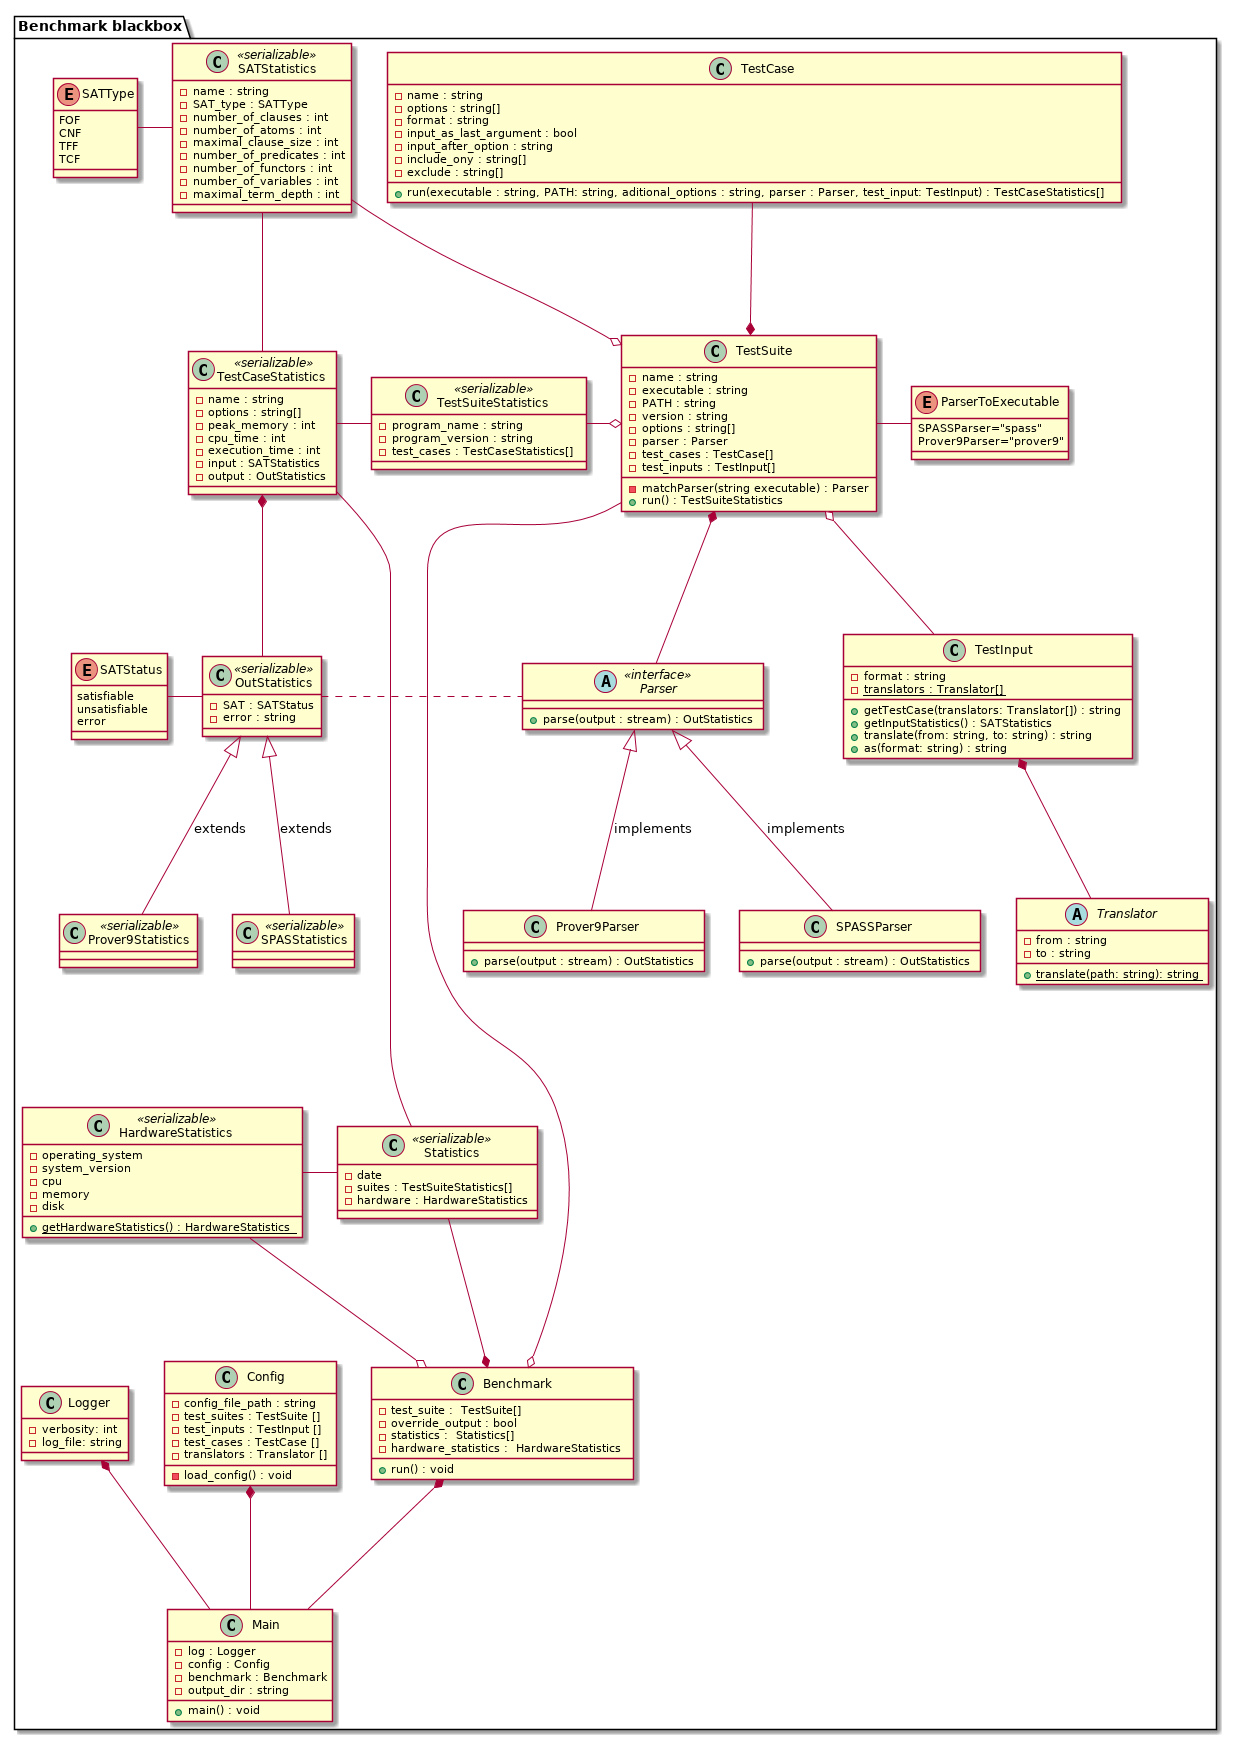
\includegraphics[width=0.9\textwidth]{benchmark/class_diagram.png}
  \caption{Diagram klas}
\end{figure}

\begin{figure}[H]
  \centering
  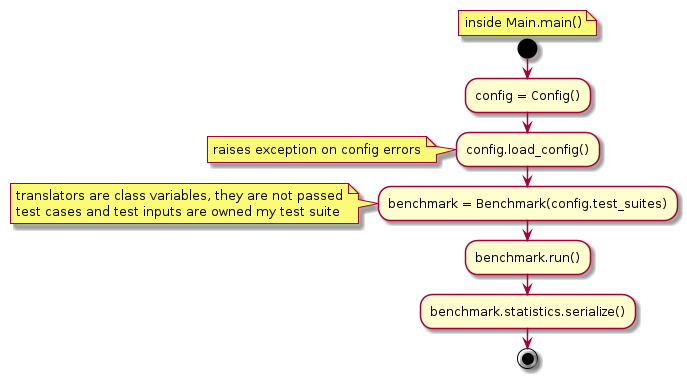
\includegraphics[width=\textwidth]{benchmark/activity_diagrams/main_run.png}
  \caption{Diagram aktywności}
\end{figure}

\begin{figure}[H]
  \centering
  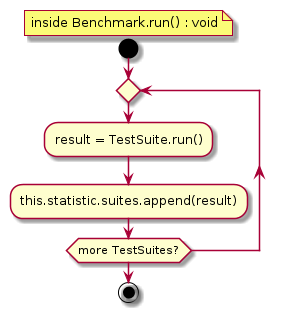
\includegraphics[width=0.8\textwidth]{benchmark/activity_diagrams/benchmark_run.png}
  \caption{Diagram aktywnośći}
\end{figure}

\begin{figure}[H]
  \centering
  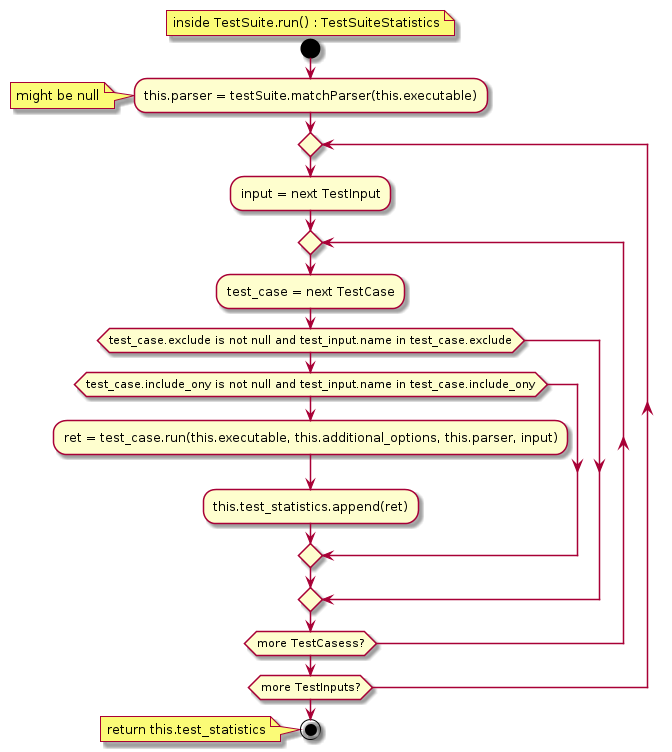
\includegraphics[width=\textwidth]{benchmark/activity_diagrams/test_suite_run.png}
  \caption{Diagram aktywnośći}
\end{figure}

\begin{figure}[H]
  \centering
  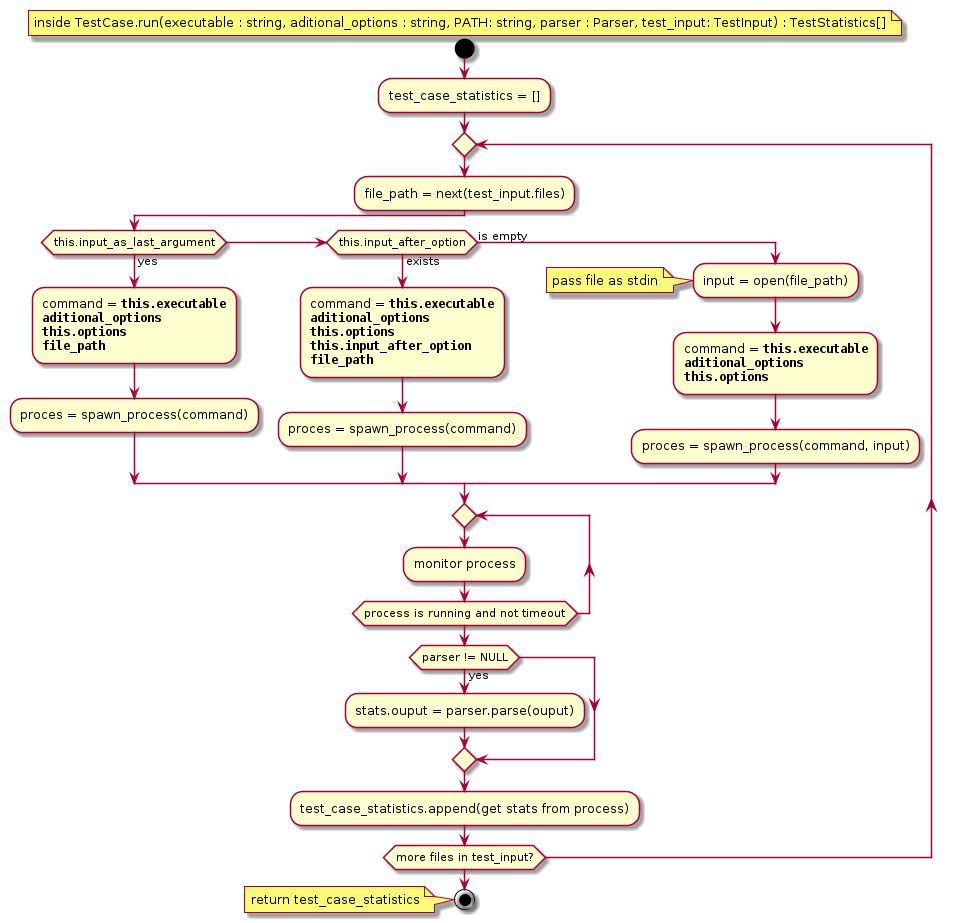
\includegraphics[width=\textwidth]{benchmark/activity_diagrams/test_case_run.png}
  \caption{Diagram aktywnośći}
\end{figure}

\section{Generator formuł logicznych} \label{LFG}

Losowy generator formuł SAT. Generator może generować formuły \gls{CNF} oraz \gls{k-SAT}. Generator może generować formuły w formacie DIMACS oraz TPTP.

\begin{figure}[H]
  \centering
  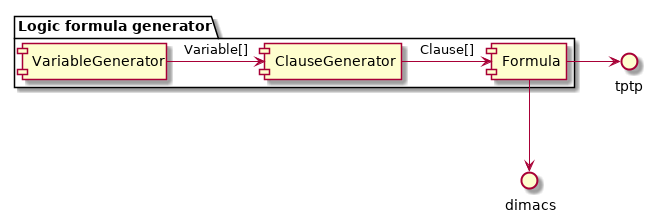
\includegraphics[scale=0.7]{logic-formula-generator/components.png}
  \caption{Komponenty generatora CNF}
\end{figure}

\begin{figure}[H]
  \centering
  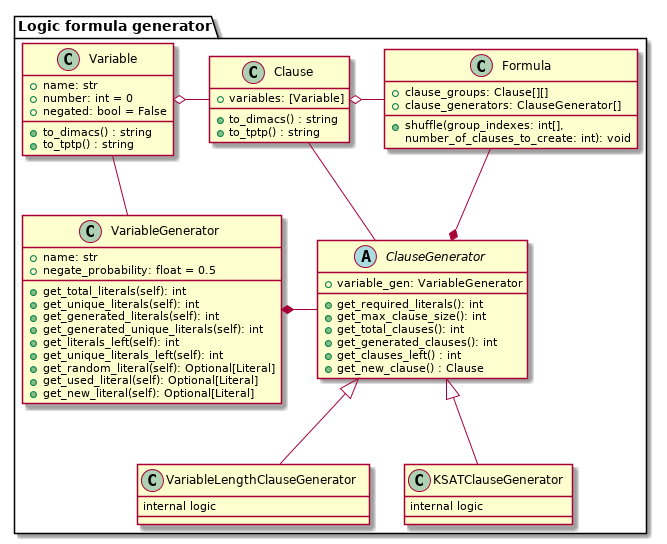
\includegraphics[scale=0.7]{logic-formula-generator/cnf_class_diagram.png}
  \caption{Diagram klas generatora CNF}
\end{figure}

\noindent
Założenia ogólne:
\begin{itemize}
  \item na jedną formułę, składa się $w$ niezależnych grup kauzul ($w$ z przedziału $[1, \infty]$). Wygenerowanie jednej grupy klauzul polega na ponownym uruchomieniu generatora z innymi parametrami. Przy czym:
    \begin{itemize}
      \item grupa klauzul nie współdzieli zbioru zmiennych
      \item grupa może posiadać całkowicie inne parametry sterujące
    \end{itemize}
  \item po wygenerowaniu, grupa klazul może być wymieszana z inną grupą klauzul. Mieszanie polega na:
    \begin{itemize}
      \item utworzeniu nowych klauzul bazując na zmiennych występujących w obu grupach - wprowadza to nowe zależności między istniejącymi już zmiennymi
    \end{itemize}
\end{itemize}

\noindent
Szczegóły implementacyjne:
\begin{itemize}
  \item logika generatora (backend) używa ogranieczeń sztywnych. Na przykład, generator zmiennych musi wygenerować \textbf{dokładnie} $n$ zmiennych, generator klauzul musi wygenerować \textbf{dokładnie} $m$ klauzul itp.
  \item ograniecznia miękkie, tzn. wygeneruj formułę z \textbf{około} $n$ zmiennych i \textbf{około} $m$ klauzul, uzyskiwane są przez wygenerowanie dokładnych warości na frontendzie i uruchomienie generatora z dokładnymi wartościami
  \item generatory są obiektami tylko do odczytu
\end{itemize}

\subsection{Generator zmiennych (\textit{VariableGenerator})}

Generator zmiennych ma za zadanie podanie dokładnie $n$ zmiennych, w tym $m$ różnych.

\noindent
Parametry sterujące:

\begin{itemize}
  \item nazwa zmiennej
  \item $m$ - ilość różnych zmiennych
  \item $n$ - ilość zmiennych do wygenerowania, ilość różnych zmiennych jest mniejsza lub równa ilości zmiennych
  \item prawdopodobieństwo zanegowania zmiennej
\end{itemize}

\noindent
Ograniczenia:
\begin{enumerate}
  \item prawdopodobieństwo zanegowania jest z zakresu $[0,1]$
  \item ilość zmiennych jest większa lub równa niż ilość różnych zmiennych $n>=m$
\end{enumerate}

\subsection{Generator klauzul (\textit{ClauseGenerator})} \label{ClauseGenerator}

Bazując na zmiennych podanych przez generator zmiennych, generuje dokładnie $k$ klauzul. Generator zmiennych musi zostać całkowicie wyczerpany. Klauzule które pochodzą z jednego generatora, nazywane są grupą klauzul.

\noindent
Parametry sterujące:
\begin{itemize}
  \item generator zmiennych
  \item ilość klauzuj do wygenerowania
  \item maksymalny rozmiar klauzuli
\end{itemize}

\noindent
Ograniczenia:
\begin{enumerate}
  \item na klauzulę przypada co najmniej jedna zmienna
  \item ilość zmiennych wymaganych przez generator klauzul musi być większa niż ilość zmiennych dostaczanych przez generator zmiennych (cały generator zmiennych musi zostać skonsumowany)
  \item każdy literał w pojedyńczej kaluzuli jest różny - nie może wystąpić: $(p1 \lor p1) \land (p1 \lor p2)$
  \item każda klauzula jest różna - nie może wystąpić: $(p1 \lor p2) \land (p1 \lor p2)$
\end{enumerate}

\subsection{Formuła (\textit{Formula})}

Formuła powstaje w wyniku kilkukrotnego uruchomiania generatora klauzul \ref{ClauseGenerator}. Zbiera ona wszystkie grupy klauzul i umożliwia mieszanie ich.

\subsection{Algorytm generowania CNF}

\begin{figure}[H]
  \centering
  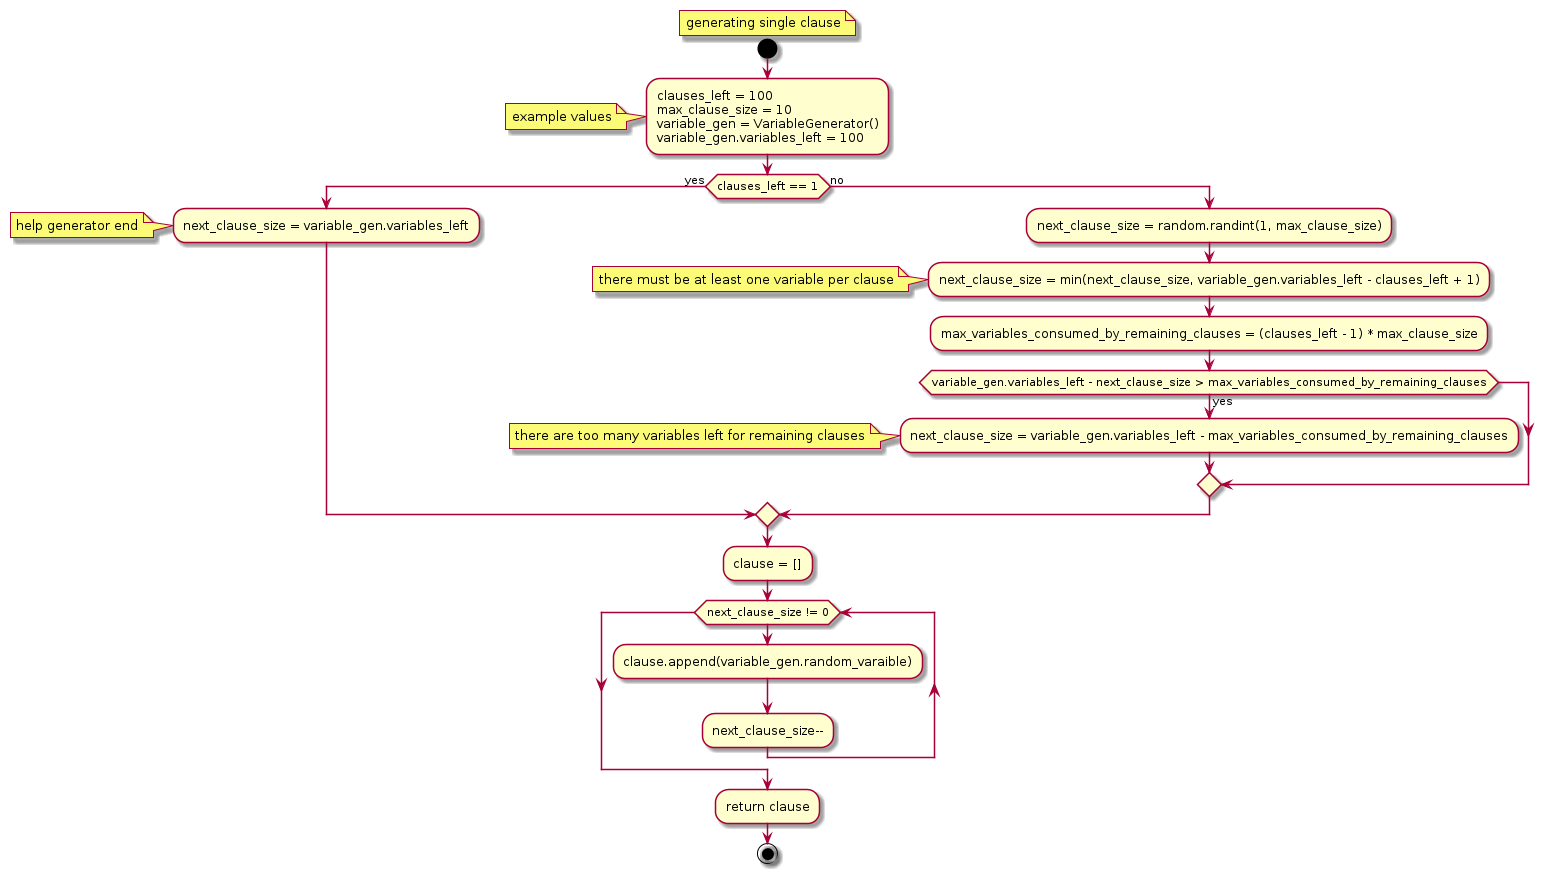
\includegraphics[width=\textwidth]{logic-formula-generator/clause_generator.png}
  \caption{Algorytm generowania pojedyńczej klauzuli}
\end{figure}

\begin{figure}[H]
  \centering
  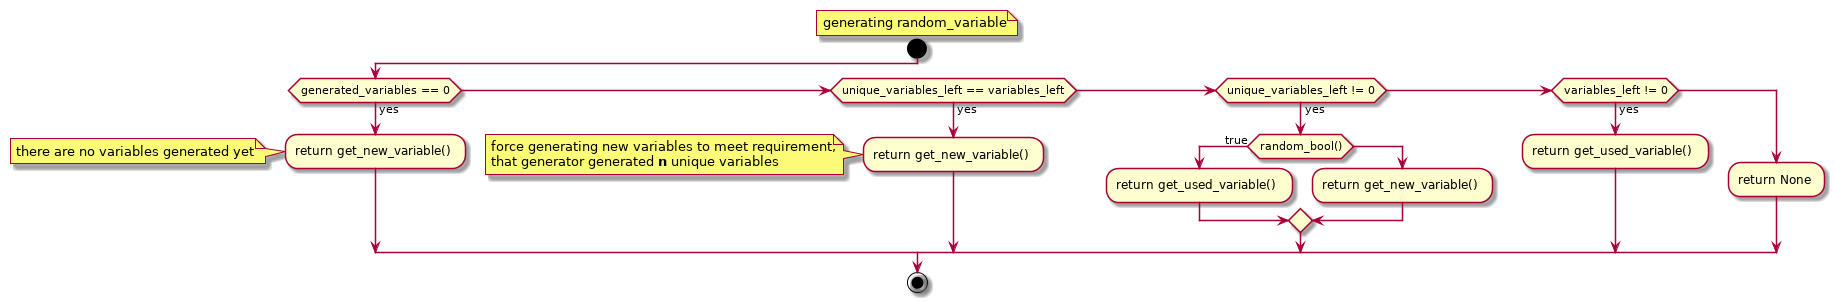
\includegraphics[width=\textwidth]{logic-formula-generator/variable_generator.png}
  \caption{Algorytm generowania losowej zmiennej}
\end{figure}

\newpage

\section{Rachunek zdań - nazewnictwo w kontekście DIMACS}

\textbf{Literał}
to zmienna lub jej zanegowanie

\textbf{Zmienna}
to ciąg znaków alfanumerycznych

\textbf{Klauzula}
to zbiór literałów połączonych logicznym znakiem \textit{i} $\land$

\begin{minted}{text}
c DIMACS CNF formula example 1
c
p cnf 3 2
1 -3 0
2 3 -1 0

c powyższa formuła składa się z:
c 2 klauzuli
c 3 zmiennych: [1,2,3]
c 5 literałów
\end{minted}

\section{Logika pierwszego rzędu - nazewnictwo w kontekście TPTP}

\textbf{Term}
to zmienna, stała lub wynik działania funktorów na zmiennych i stałych

\textbf{Atom}
to wyrażenie logiczne, które nie może zostać rozbite na składowe

% \textbf{Equolity atom}

\textbf{Literał}
to atom lub jego zaprzeczenie

\textbf{Zmienna}
to atom, który zaczyna się z dużej litery. Zmienna ma zasięg klauzulu. Tzn. jeśli zmienna $A$ pojawi się w jednej klazuli kilkukrotnie jest to dalej jedna zmienna.

\textbf{Zmienna singletonowa}
to zmienna użyta tylko raz w klauzuli

\textbf{Unit clause}
to klauzula, która posiada tylko jeden atom

\textbf{Horn clause}
to klaulula, która posiada co najmniej jeden pozytywny literał

\textbf{RR clause} - ??

\textbf{Predykat}
jest to operator logiczny, który zwraca prawdę lub fałsz. Predykat operuje na określonej liczbie termów. Liczba ta jest stała i nazywana argumentowością predykatu (\textit{arity}).

\textbf{Funktor}
oprator logiczny, który zwraca term. Funktor posiada określoną argumentowość.

\textbf{Constant functor}
to funktor o argumentowości 0

\textbf{Klauzula}
jest to zbiór termów połączonych dysjunkcją ($\lor$)

% \textbf{Kwantyfikator} not in scope

\begin{tptpcode}
% TPTP CNF formula example 1
cnf(simple_clause_1, axiom,
    ( p(f,f) | ~p(a,b) | p(X, V) | pp(X) )).
 
% powyższa formuła składa się z:
% 1 klauzuli: w tym 0 jednostkowa, 1 Horn
% 4 literały: [p(f,f), ~p(a,b), p(X, V), pp(X)]
% 4 atomy: [p(f,f), p(a,b), p(X, V), pp(X)]
% 2 predykatów: [p, pp] o argumentowości 1: [pp] i 2: [p]
% 3 funktorów: [f, a, b] o argumentowości 0 - funktory stałe
% 2 zmiennych: [X, V] w tym 1 zmienna singletonowo
\end{tptpcode}

\begin{tptpcode}
% TPTP CNF formula example 2
cnf(simple_clause_1, axiom,
    ( p(f,f) | ~p(a,b) | p(X, V) | pp(X) )).

cnf(simple_clause_2, axiom,
    ( pp(f) | pp(X) )).

cnf(simple_clause_3, axiom,
    ( ppp )).

% powyższa formuła składa się z:
% 3 klauzuli, w tym 1 klauzula jednostkowa, 3 Horn
% 4 literały: [p(f,f), ~p(a,b), p(X, V), pp(X)]
% 4 atomy: [p(f,f), p(a,b), p(X, V), pp(X)]
% 3 predykatów: [p, pp, ppp] o argumentowości 0: [ppp], 1: [pp] i 2: [p]
% 3 funktorów: [f, a, b] o argumentowości 0 - funktory stałe
% 3 zmiennych: [X, V] w tym 2 zmienne singletonowe
\end{tptpcode}

\begin{tptpcode}
% TPTP CNF formula example 3
cnf(simple_clause_1, axiom,
    ( p(f,f) | ~p(f,f) )).

% powyższa formuła składa się z:
% 1 klauzuli, w tym 0 jednowtkowa, 1 Horn
% 2 literały: [p(f,f), ~p(f,f)]
% 1 atomy: [p(f,f)]
% 1 predykatu: [p] o argumentowości 2
% 1 funktorów: [f] o argumentowości 0 - funktor stały
% 0 zmiennych
\end{tptpcode}

\begin{tptpcode}
% TPTP CNF formula example 4
cnf(simple_clause_1, axiom,
    ( p(f,f) | ~p(f,f) )).

cnf(simple_clause_2, axiom,
    ( ~p(f,f) )).

% powyższa formuła składa się z:
% 2 klauzuli, w tym 1 jednostkowa, 1 Horn
% 2 literały: [p(f,f), ~p(f,f)]
% 1 atomy: [p(f,f)]
% 1 predykatu: [p] o argumentowości 2
% 1 funktorów: [f] o argumentowości 0 - funktor stały
% 0 zmiennych
\end{tptpcode}

\newpage
\section{Zestaw testowy}


\noindent
\textbf{Problem:} Jak ilość atomów wpływa na czas wykonania?

Zestaw to formuły CNF różnej długości
\begin{itemize}
  \item liczba klauzul to 100, 200, 500, 1000, 2500, 5000
  \item stosunek atomów do klauzul wynosi 2, 3, 4, 5, 10 (2 oznacza, że jeśli liczba klauzul to 100, wtedy liczba atomów to 200)
  \item maksymalna długość klauzuli to ilość wszystkich zmiennych / ilość klauzul
\end{itemize}

\noindent
\textbf{Problem:} Jak stosunek atomów bezpieczeństwa do atomów żywotnościowych wpływa na czas wykonania?

Zestaw to formuły CNF różnej długości
\begin{itemize}
  \item liczba klauzul to 100, 200, 500, 1000, 2500, 5000
  \item stosunek atomów bezpieczeństwa do atomów żywotnościowych wynosi 2, 3, 4, 5, 10
  \item maksymalna długość klauzuli to ilość wszystkich zmiennych / ilość klauzul
\end{itemize}

\noindent
\textbf{Problem:} Jak udział k-SAT i zmiennych wpływa na czas wykonania?
\newline
\textbf{Hipoteza:}
\begin{enumerate}
  \item obecność co najmniej jednej klauzul k-SAT, gdzie k dąży do 1, sprzyja szybkiemu rozwiązaniu problemu
  \item obecność co najmniej jednej klauzul k-SAT, gdzie k dąży do $\infty$, znacząco spowalnia rozwiązanie problemu
  \item im większa obecność klazul z dużym k, tym większy czas wykonywania
\end{enumerate}

Zestaw skupia się na k-SAT:
\begin{itemize}
  \item liczba klauzul to 100, 200, 300, 400, 500, 1000, 2000, 3000, 4000, 5000
  \item klauzule są postaci:
    \begin{itemize}
      \item 1,5,10,20-SAT -- kada z nich stanowi 25\% wszystkich klauzul (po równo)
      \item 1,5,10,20-SAT -- 1-SAT to 1\% (minimum 1), 5,10,20-SAT po równo
      \item 1,5,10-SAT -- po równo
      \item 1,5,10,20-SAT -- 20-SAT to 1\% (minimum 1), 1,5,10-SAT po równo
      \item 5,10,20-SAT -- po równo
    \end{itemize}
\end{itemize}

% \noindent
% \textbf{•}f{Problem:} Jak zmiesznie klauzul i zmiennych wpływa na czas wykonania? TODO nie wiemy co badać

% Zestaw stworzony jest z mieszania niezależnych grup klauzul (grupy nie współdzielą zmiennych).  Mieszanie polega na dodaniu klauzul, które operują na wspólnym zbiorze zmiennych z obu grup.
% \begin{itemize}
%   \item grupa posiada 50 zmiennych
%   \item liczba grup to 5, 10, 15, 20
%   \item mieszanie:
%     \begin{itemize}
%       \item bez mieszania (grupa kontrolna)
%       \item weź grupy o numerach (1, 2) i stwórz jeszcze 10 klazul, ilość zmiennych jest losowa. Powtórz to samo dla grup $(n,n+1)$ - jedna grupa jest powiązana tylko z jedną grupą
%       \item inne kombinacje, co chcemy z tego wywnioskować?
%     \end{itemize}
%   \item w wyniku zmieszania powstaje od 2 do 25 nowych klauzul. Do stworzenia klauzul użytych jest od 20 do 50 literałów
% \end{itemize}
%
\section{Wnioski}

Celem projektu było zbadanie które z czynników formuł logicznych wpływają najbardziej na działanie proverów SPASS oraz Prover9. Aby odpowiedzieć na to pytanie napisany został generator formuł o zadanych parametrach które następnie były przepuszczane przez provery z użyciem strategii blackbox. Na wyjściu otrzymane zostały pliki JSON z parametrami wejścia takimi jak: liczba klauzul, atomów, predykatów, funktorów, zmiennych oraz parametrami wyjścia: czasem wykonania, maksymalnym zużyciem pamięci (peak memory) oraz statusem (spełnialna, niespełnialna, timeout). W celu ograniczenia czasu wykonywania się benchmarków wprowadzono górną granicę czasu na każdy test case: 300 sekund.

\subsection{Zestaw 1}

Jak widać na wykresach załączonych poniżej według oczekiwań największy wpływ na czas wykonywania/używaną pamięć największy wpływ ma ilość klauzul.
Zarówno na czas wykonania oraz na zużytą pamięć zauważalny wpływ ma również stosunek liczby atomów do klauzul, pierwszy taki skok możemy zauważyć w Proverze9 dla test case'ów o 200 klauzulach, gdzie test case o 2000 atomach zakończył się timeout'em przy niewielkim wzroście pamięci. Zwiększenie się czasu wykonywania oraz zużytej pamięci widać bardzo dobrze dla test case'ów Provera9 o 500 oraz 1000 klauzulach. Dla 2500 klauzul i stosunku atomy/klauzule większego lub równego od 4 oraz dla wszystkich testcase'ów o 5000 klauzulach benchmark kończył się timeoutem. Warto zauważyć coraz bardziej stromy wzrost zużytej pamięci dla większych ilości klauzul dla Provera9. Dla SPASS już od najmniejszych pod względem ilości klauzul test case'ach zużycie pamięci jest znacząco większe nawet od największych pod względem ilości klauzul test case'ach w Proverze9 co przemawia na korzyść tego provera.

\begin{figure}[H]
  \centerline{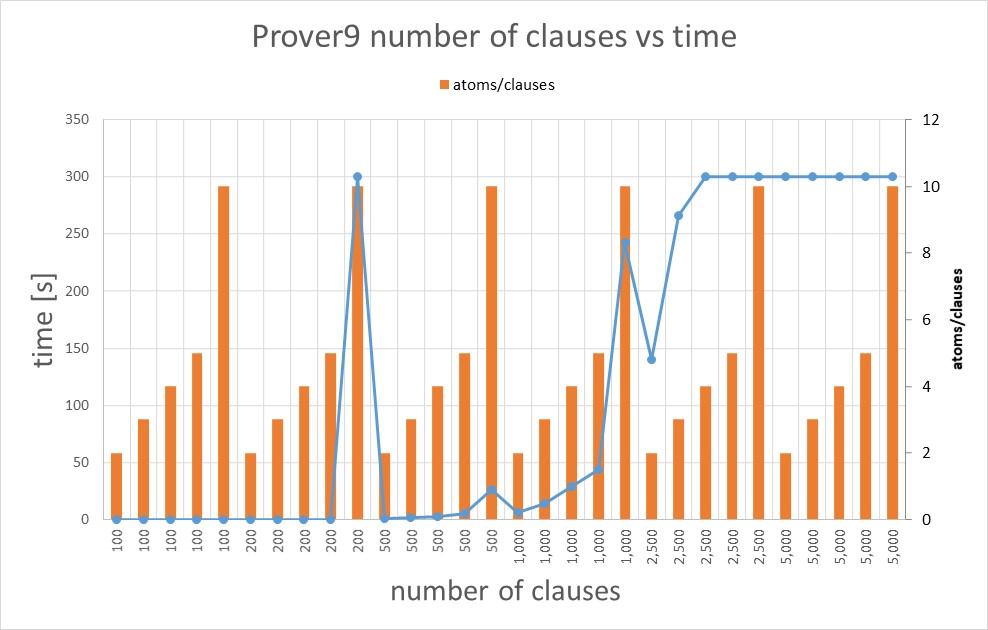
\includegraphics[width=0.9\textwidth]{outputs/set1/set1 charts/01 Prover9 number of clauses vs time.jpg}}
  \caption{Prover9 zestaw 1 liczba klauzul vs czas}
\end{figure}

\begin{figure}[H]
  \centerline{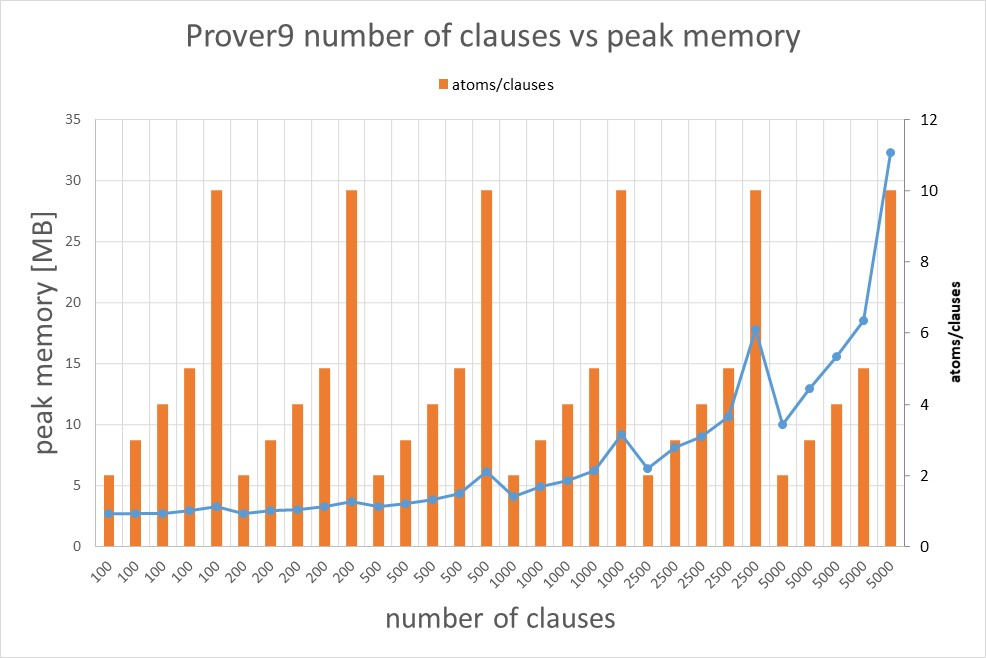
\includegraphics[width=0.9\textwidth]{outputs/set1/set1 charts/02 Prover9 number of clauses vs peak memory.jpg}}
  \caption{Prover9 zestaw 1 liczba klauzul vs pamięć}
\end{figure}

\begin{figure}[H]
  \centerline{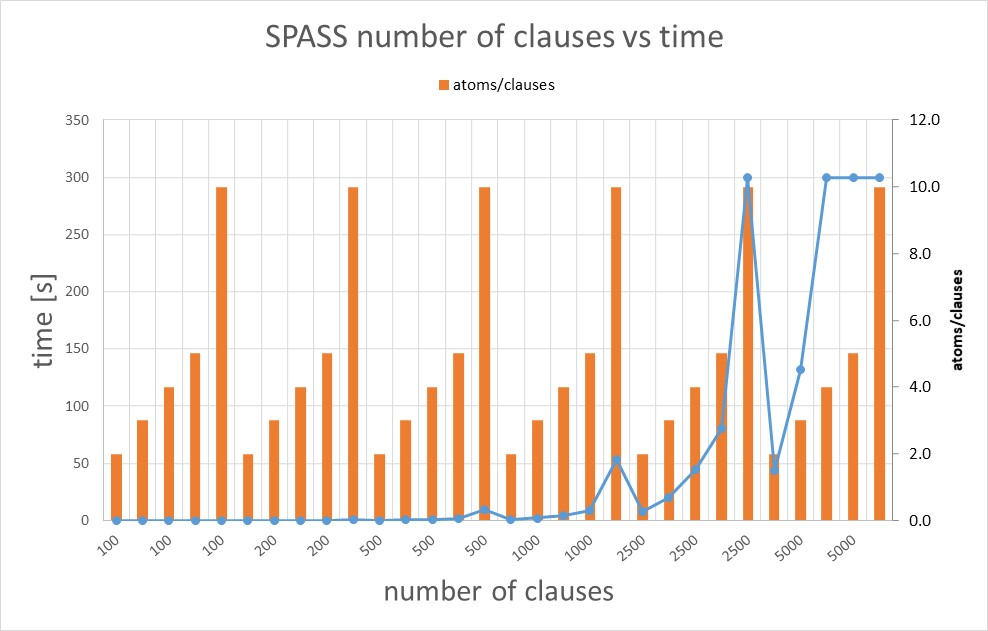
\includegraphics[width=0.9\textwidth]{outputs/set1/set1 charts/11 SPASS number of clauses vs time.jpg}}
  \caption{SPASS zestaw 1 liczba klauzul vs czas}
\end{figure}

\begin{figure}[H]
  \centerline{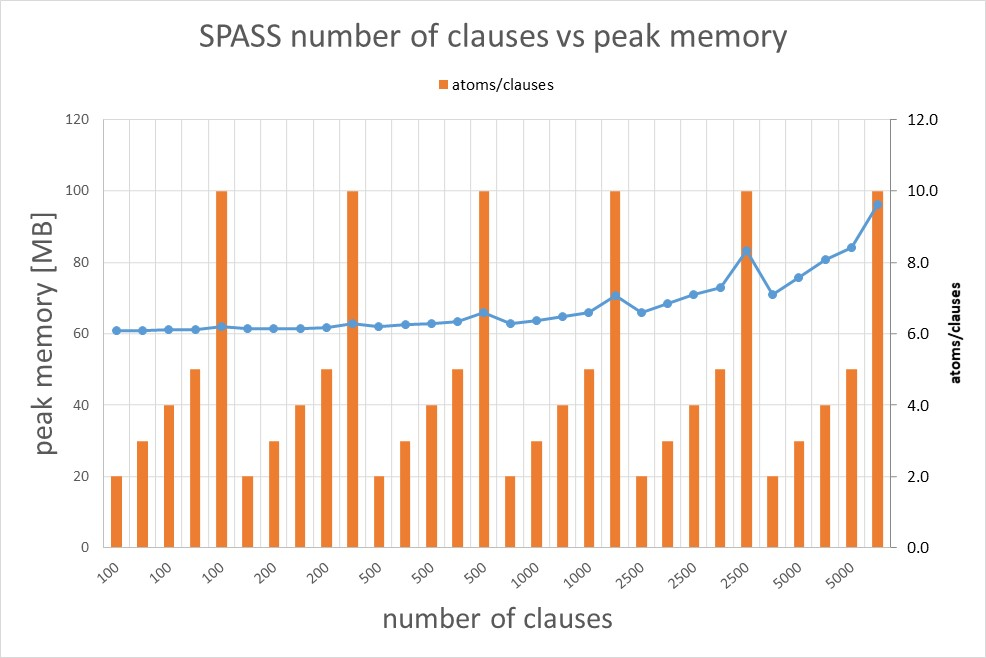
\includegraphics[width=0.9\textwidth]{outputs/set1/set1 charts/12 SPASS number of clauses vs peak memory.jpg}}
  \caption{SPASS zestaw 1 liczba klauzul vs pamięć}
\end{figure}




\subsection{Zestaw 2}

W zestawie 2 badano wpływ stosunku ilości atomów bezpieczeństwa do ilości atomów żywotności. W grupach test case'ów o tych samych ilościach klauzul zadano różne stosunki ilości atomów bezpieczeństwa do ilości atomów żywotności. Z otrzymanych wyników można wywnioskować, że zbyt nierówny stosunek tych liczb (odbiegający od 1 w obie strony) wpływa znacząco na czas wykonywania się benchmarku, wpływ ten jest większy dla Provera9 niż dla SPASS. Najlepiej widać tą zależność w Proverze9 dla test case'ów z 1000 klauzul. Tak samo jak dla zestawu 1 SPASS zużywa znacząco więcej pamięci niż Prover9 jednakże w zestawie 2 można zauważyć kilkukrotnie mniejszą ilość timeout'ów dla SPASS.

\begin{figure}[H]
  \centerline{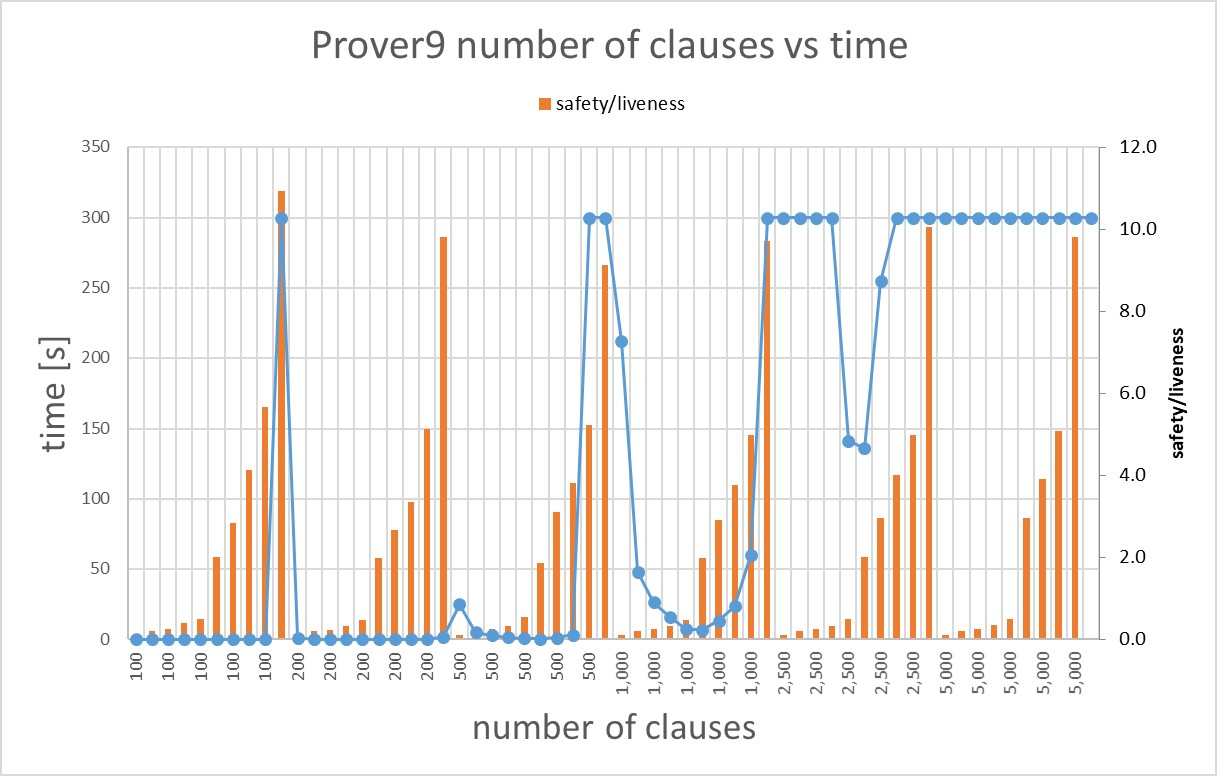
\includegraphics[width=0.9\textwidth]{outputs/set2/set2 charts/01 Prover9 number of clauses vs time.jpg}}
  \caption{Prover9 zestaw 2 liczba klauzul vs czas}
\end{figure}

\begin{figure}[H]
  \centerline{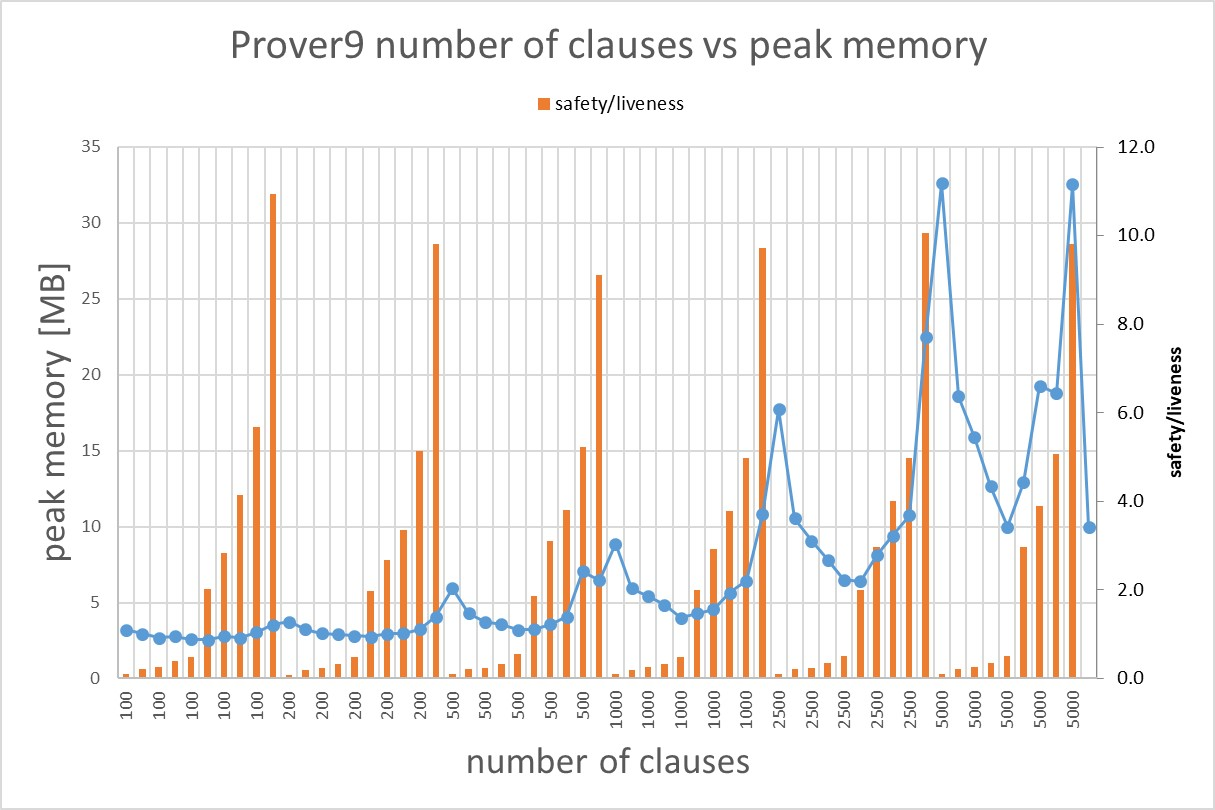
\includegraphics[width=0.9\textwidth]{outputs/set2/set2 charts/02 Prover9 number of clauses vs peak memory.jpg}}
  \caption{Prover9 zestaw 2 liczba klauzul vs pamięć}
\end{figure}

\begin{figure}[H]
  \centerline{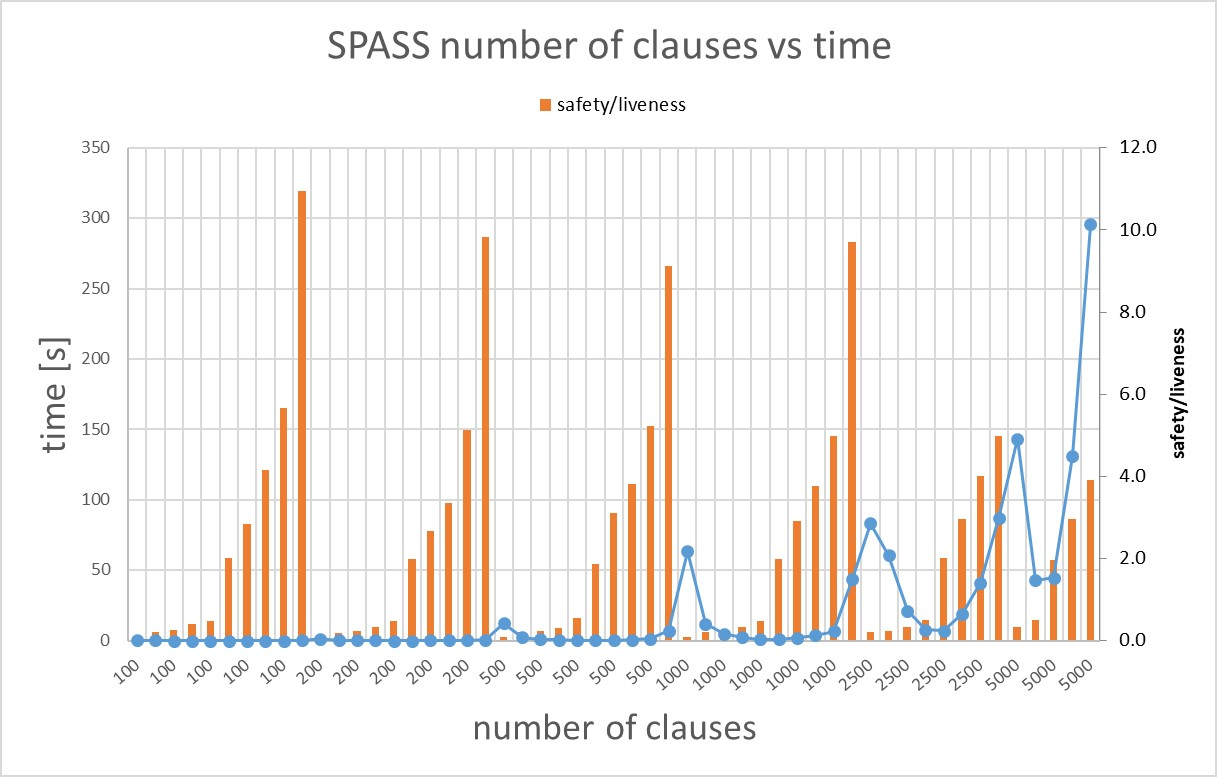
\includegraphics[width=0.9\textwidth]{outputs/set2/set2 charts/11 SPASS number of clauses vs time.jpg}}
  \caption{SPASS zestaw 2 liczba klauzul vs czas}
\end{figure}

\begin{figure}[H]
  \centerline{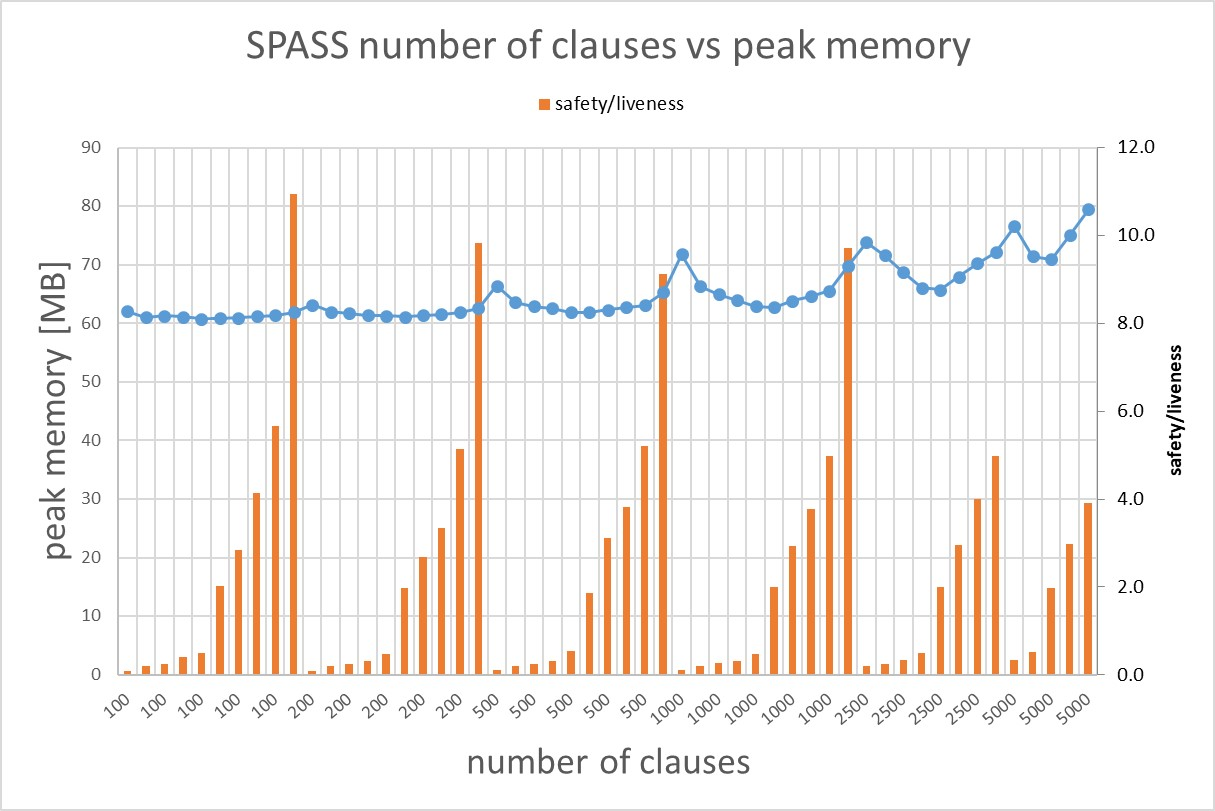
\includegraphics[width=0.9\textwidth]{outputs/set2/set2 charts/12 SPASS number of clauses vs peak memory.jpg}}
  \caption{SPASS zestaw 2 liczba klauzul vs pamięć}
\end{figure}


\subsection{Zestaw 3}

W zestawie 3 badano wpływ udziału klauzul k-SAT na czas wykonywania/pamięć w zależności od k. Zadano klauzule o różnym stopniu rozłożenia spośród wartości k $\epsilon$ \{1,5,10,20\}. Jak można było oczekiwać, test case'y o tej samej sumarycznej liczbie klauzul a o najmniejszym udziale klauzul z wysokim k miały najszybszy czas wykonywania oraz zużywały najmniej pamięci. Warto zwrócić uwagę na stopień tej zależności czyli zdecydowanę przewagę szybkości rozwiązań test case'ów o największym procentowym udziale klauzul 1-SAT, wraz ze wzrostem k czas rośnie lecz przyrost ten maleje co sugeruje zależność logarytmiczną czasu wykonania od~k. Dla Provera9 najlepiej wpływ k widać na wykresie zależności liczby klauzul od pamięci (Rys 21.), charakterystyczne są grupy trzech test case'ów o tych samych liczbach klauzul a innym rozłożeniu k. Dla SPASS wyniki dają podobne wnioski, zauważalne jest kolejny raz wysokie zużycie pamięci i niewiele mniejsza liczba timeout'ów w porównaniu do Provera9.

\begin{figure}[H]
  \centerline{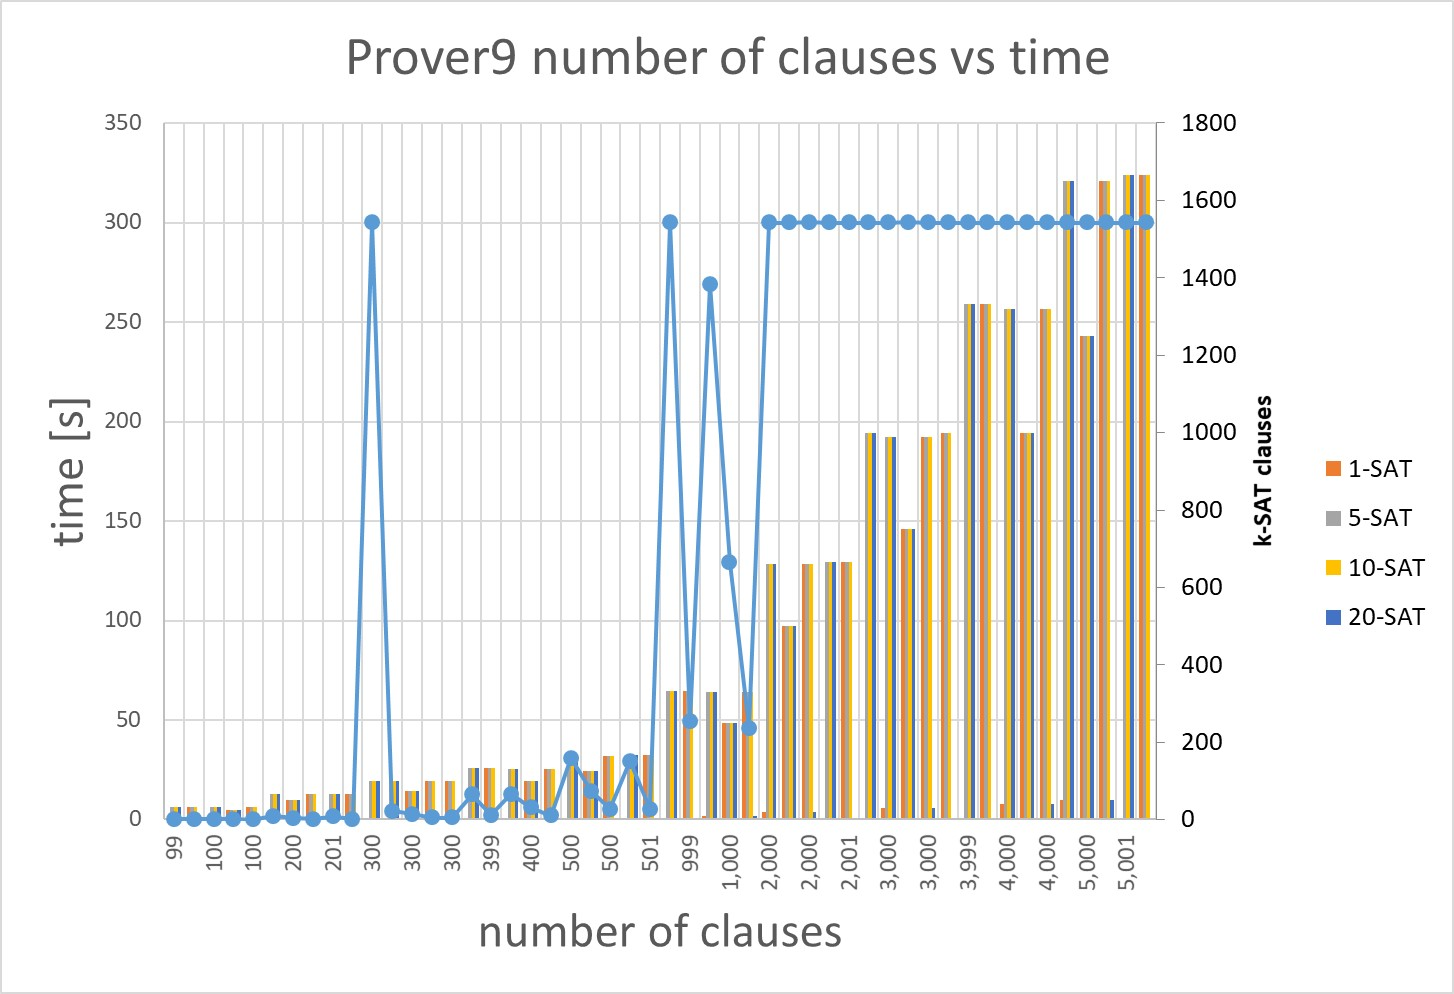
\includegraphics[width=0.85\textwidth]{outputs/set3/set3 charts/01 Prover9 number of clauses vs time.jpg}}
  \caption{Prover9 zestaw 3 liczba klauzul vs czas}
\end{figure}

\begin{figure}[H]
  \centerline{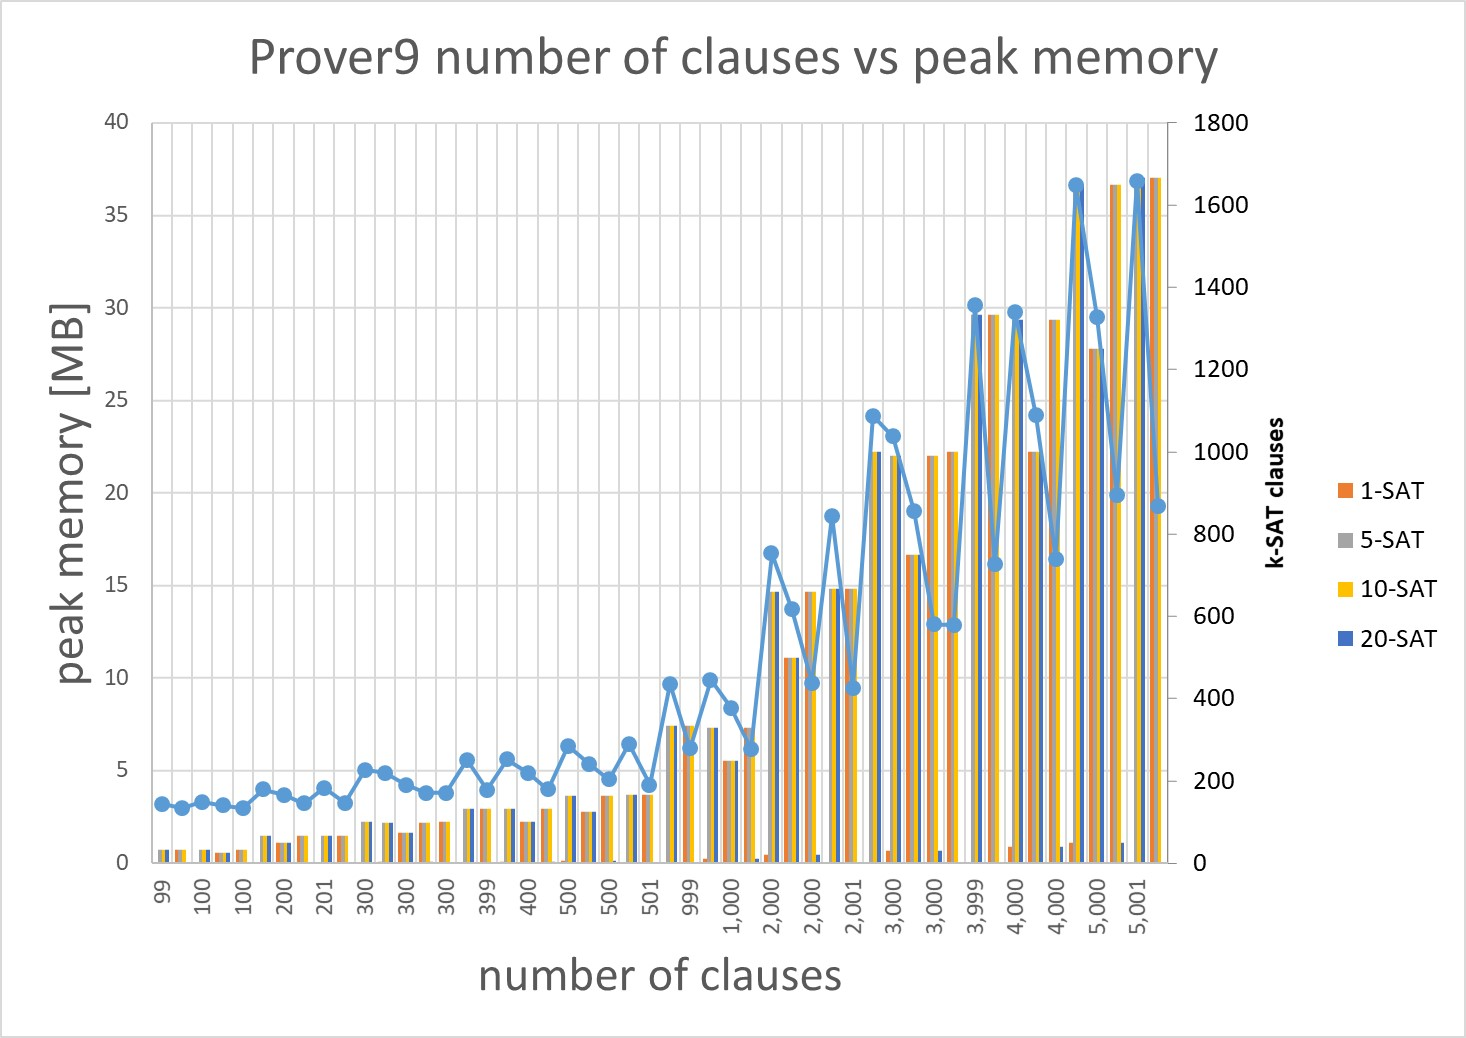
\includegraphics[width=0.85\textwidth]{outputs/set3/set3 charts/02 Prover9 number of clauses vs peak memory.jpg}}
  \caption{Prover9 zestaw 3 liczba klauzul vs pamięć}
\end{figure}

\begin{figure}[H]
  \centerline{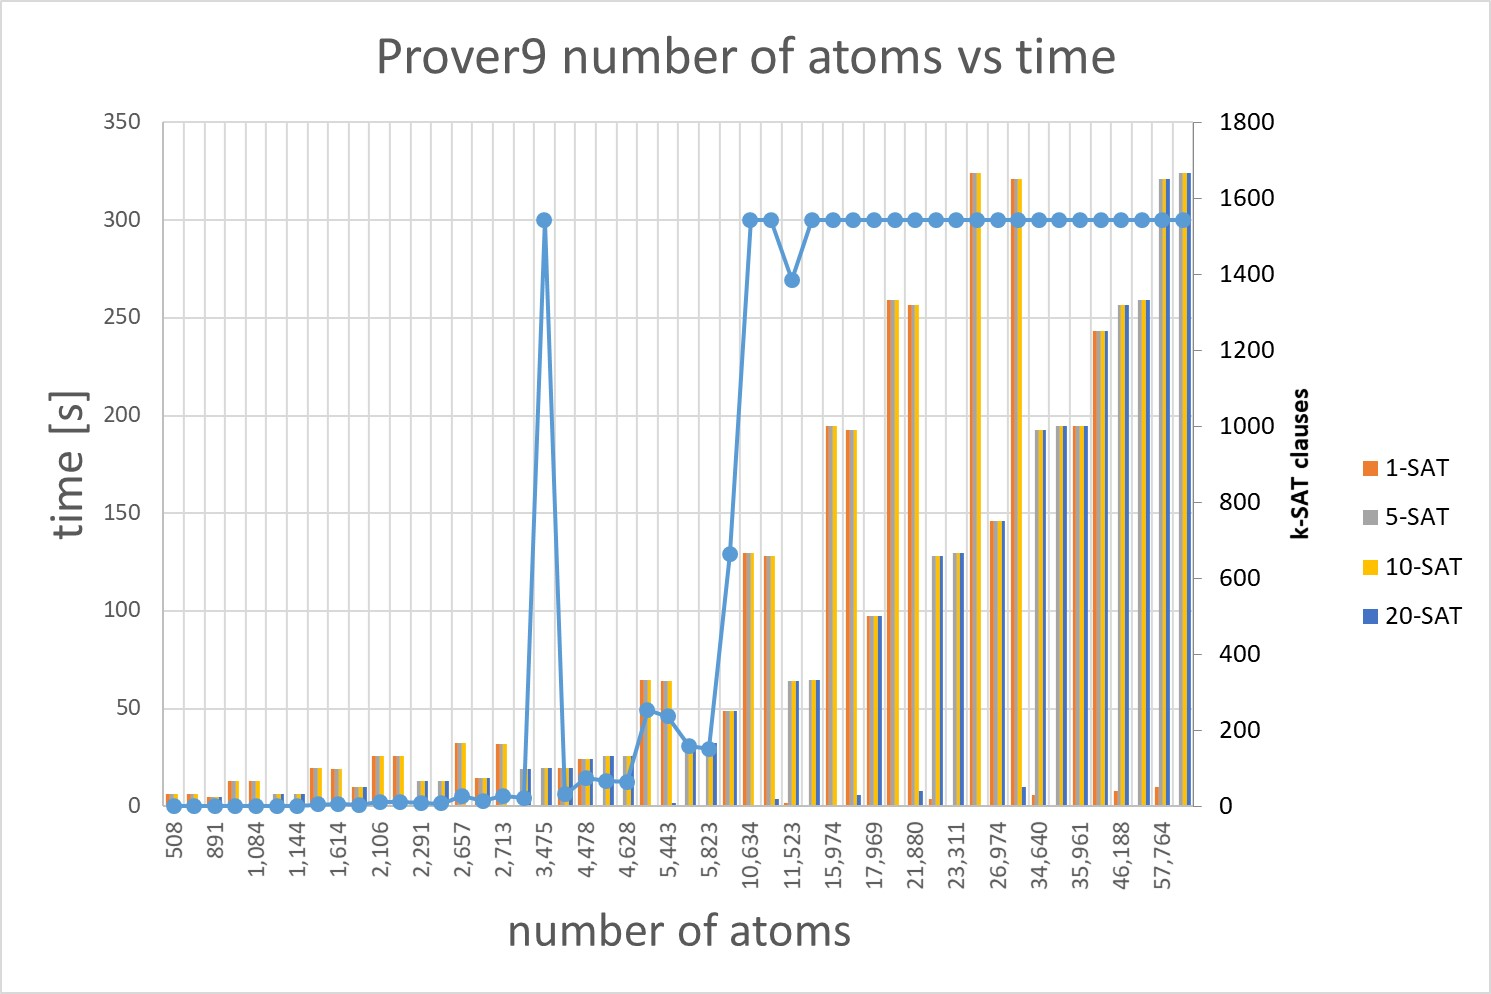
\includegraphics[width=0.9\textwidth]{outputs/set3/set3 charts/03 Prover9 number of atoms vs time.jpg}}
  \caption{Prover9 zestaw 3 liczba atomów vs czas}
\end{figure}

\begin{figure}[H]
  \centerline{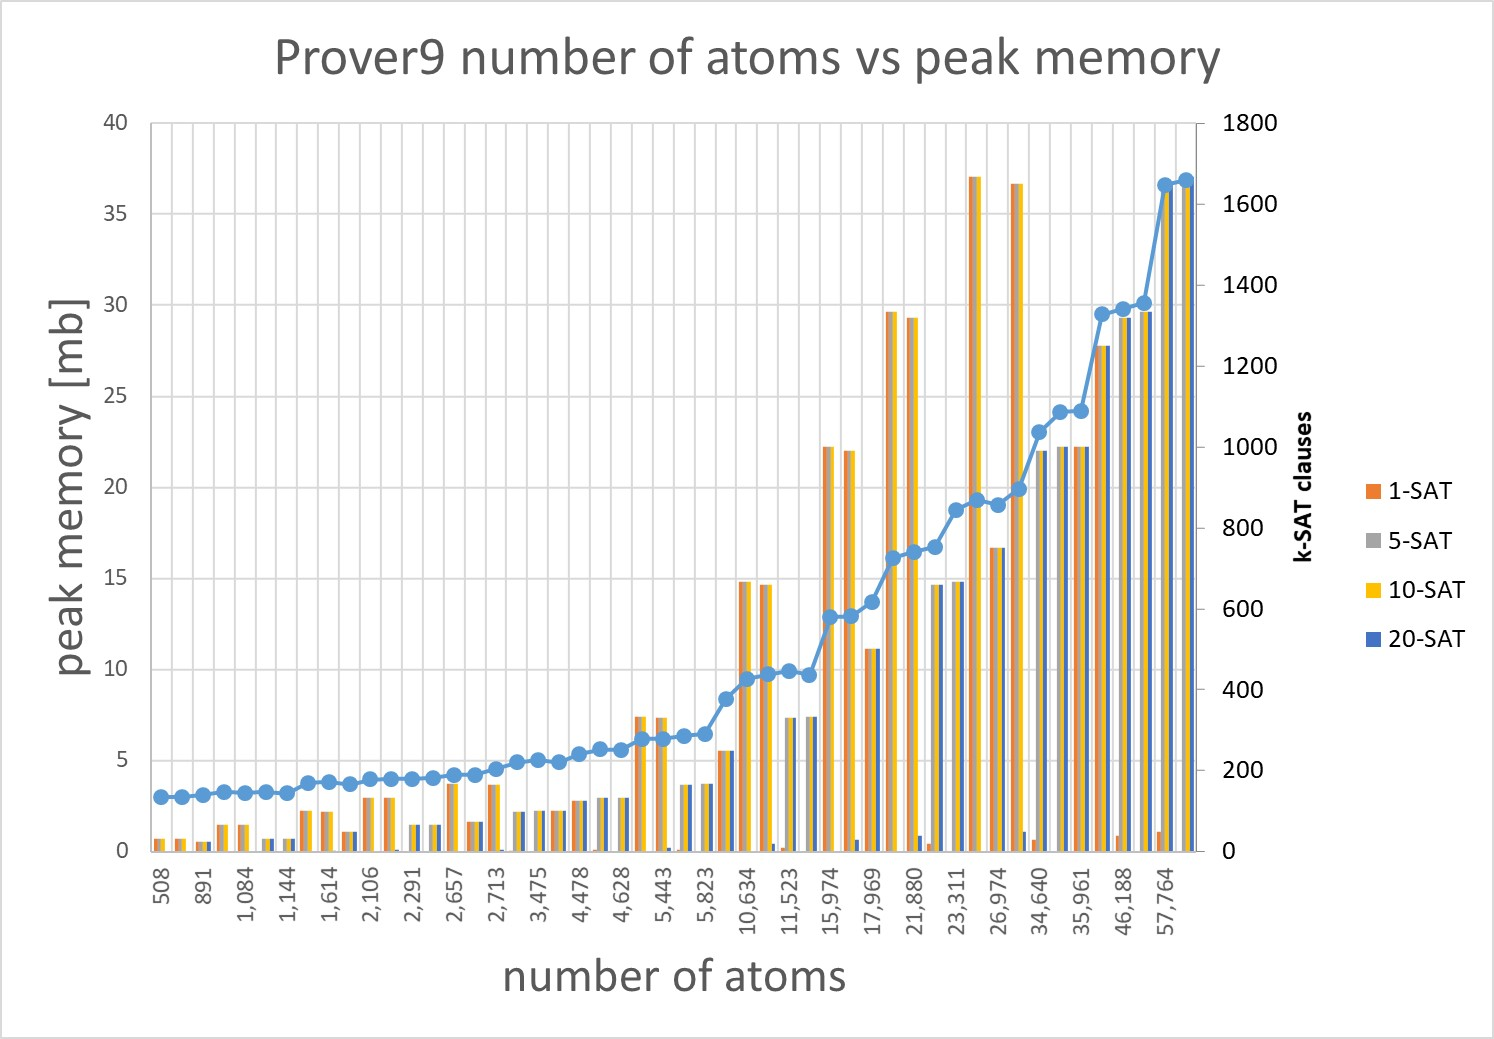
\includegraphics[width=0.9\textwidth]{outputs/set3/set3 charts/04 Prover9 number of atoms vs peak memory.jpg}}
  \caption{Prover9 zestaw 3 liczba atomów vs pamięć}
\end{figure}


\begin{figure}[H]
  \centerline{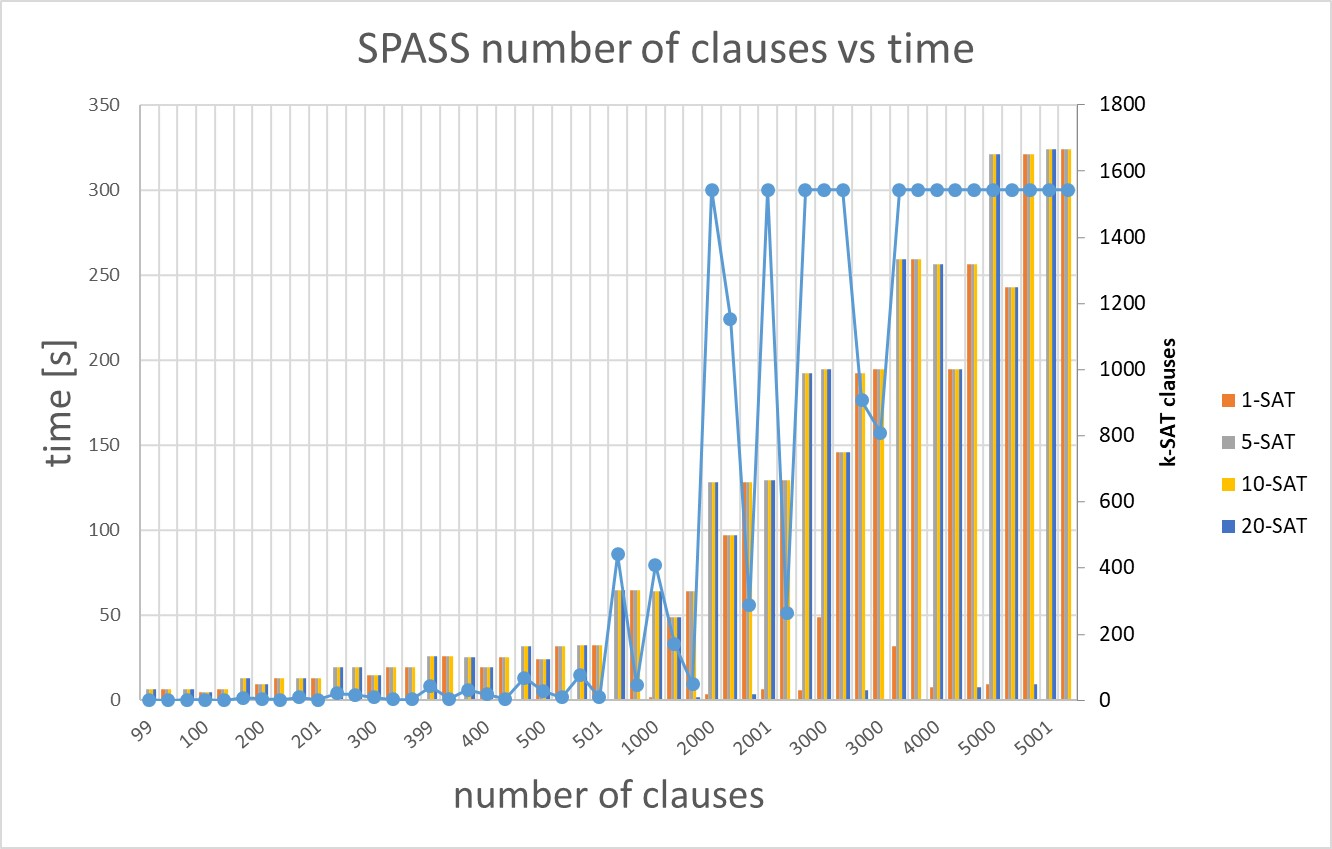
\includegraphics[width=0.9\textwidth]{outputs/set3/set3 charts/11 SPASS number of clauses vs time.jpg}}
  \caption{SPASS zestaw 3 liczba klauzul vs czas}
\end{figure}

\begin{figure}[H]
  \centerline{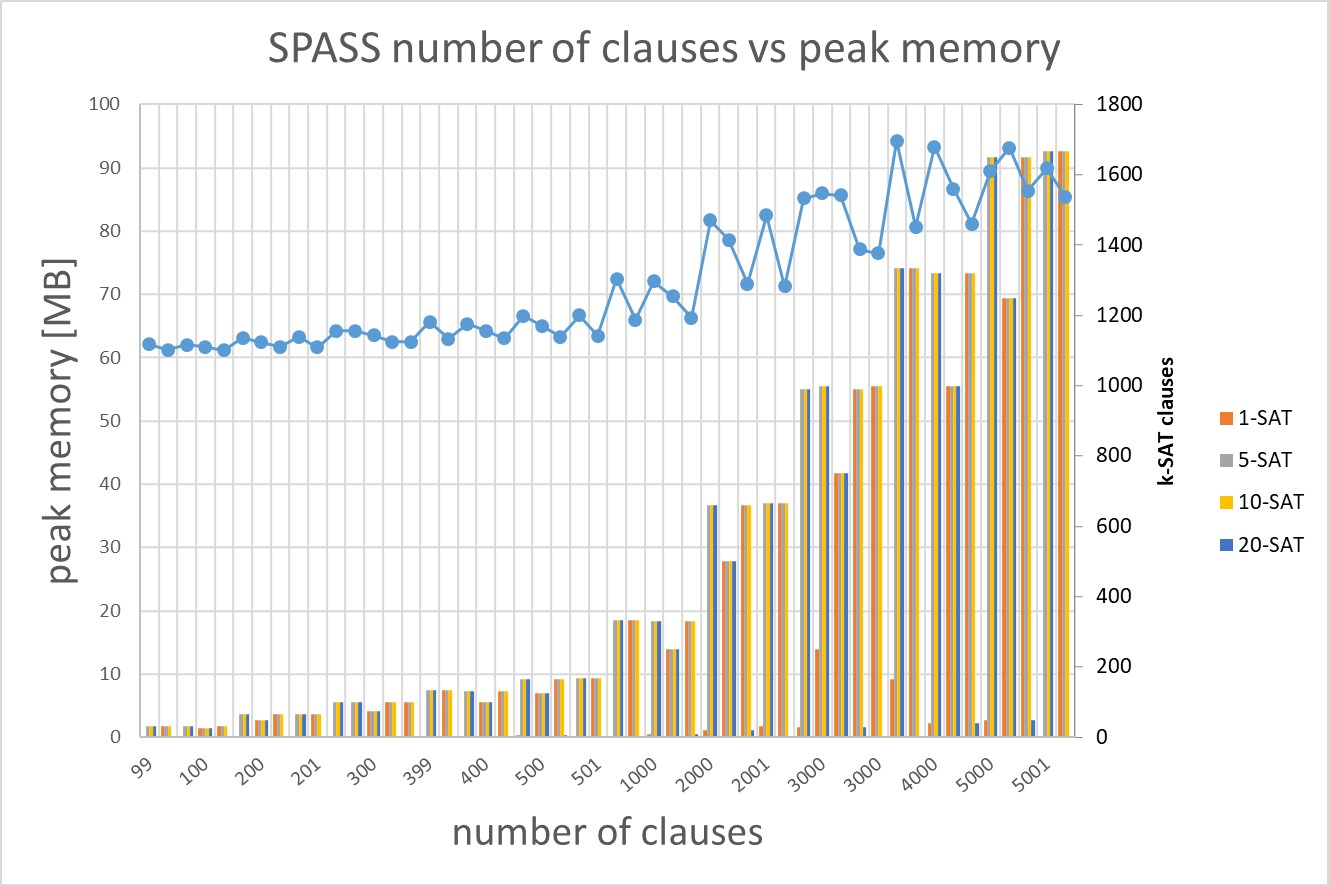
\includegraphics[width=0.9\textwidth]{outputs/set3/set3 charts/12 SPASS number of clauses vs peak memory.jpg}}
  \caption{SPASS zestaw 3 liczba klauzul vs pamięć}
\end{figure}


\begin{figure}[H]
  \centerline{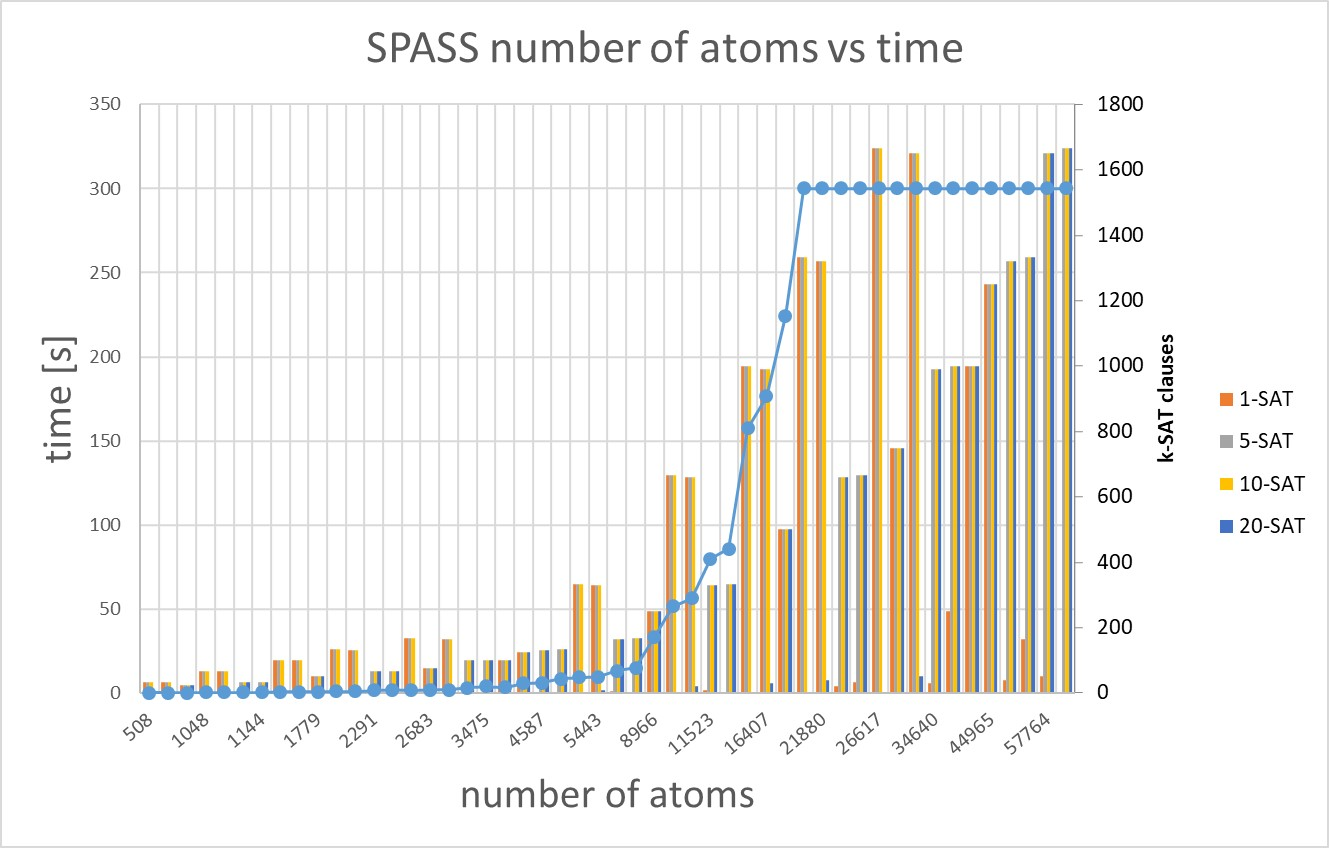
\includegraphics[width=0.9\textwidth]{outputs/set3/set3 charts/13 SPASS number of atoms vs time.jpg}}
  \caption{SPASS zestaw 3 liczba atomów vs czas}
\end{figure}

\begin{figure}[H]
  \centerline{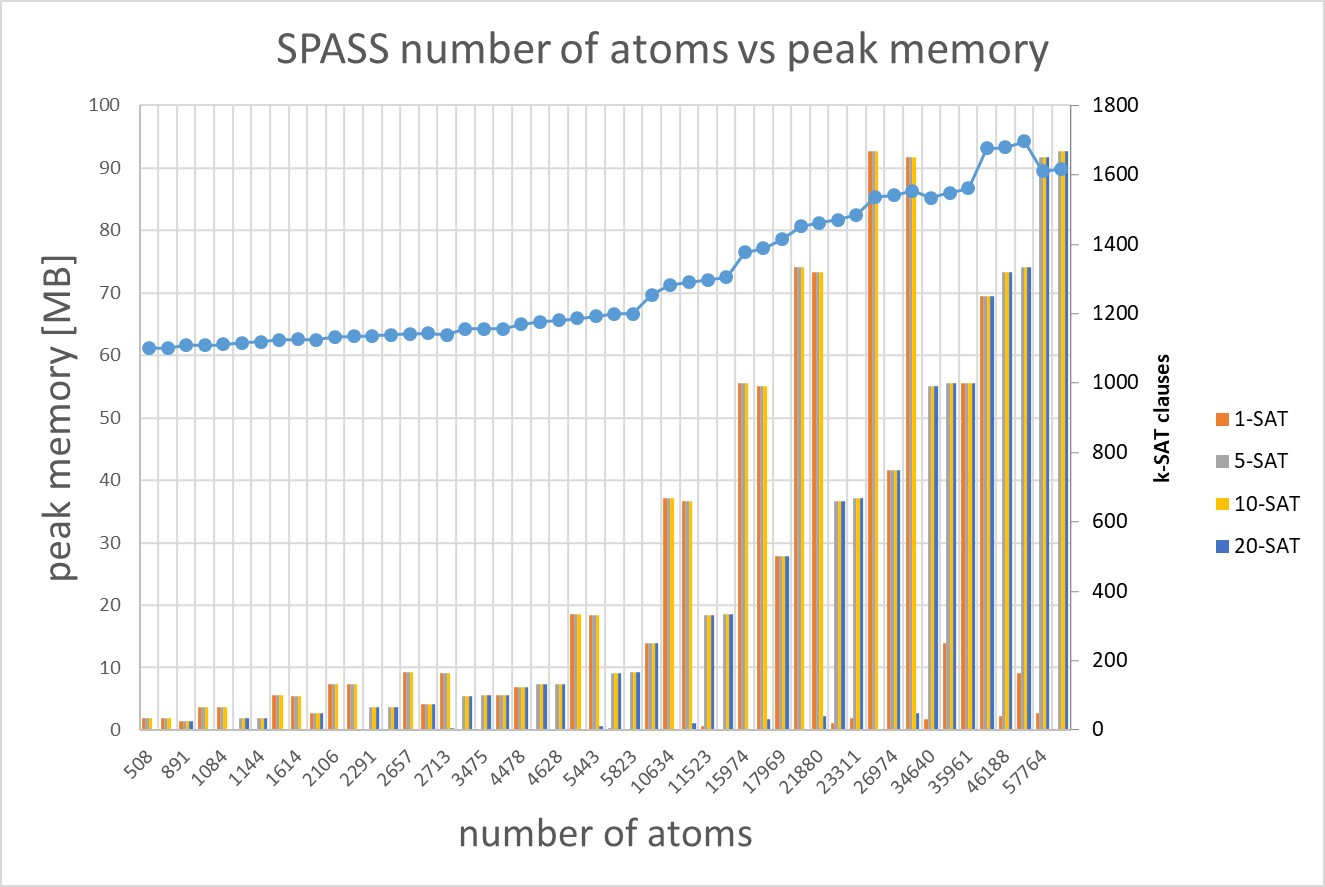
\includegraphics[width=0.9\textwidth]{outputs/set3/set3 charts/14 SPASS number of atoms vs peak memory.jpg}}
  \caption{SPASS zestaw 3 liczba atomów vs czas}
\end{figure}

\printglossary

\end{document}
